\documentclass{article}

\usepackage{NotesPackage}

\newcommand{\esc}{\overset{\text{\tiny ESC}}{=}}
\newcommand{\defeq}{\overset{\text{\tiny def}}{=}}
\newcommand{\pdvx}[1]{\partial_{x_{#1}}}
\newcommand{\divword}{\mathop{\mathrm{div}}}
\newcommand{\curlword}{\mathop{\mathrm{curl}}}
 
\newcommand{\notesVersion}{1.0}
\newcommand{\notesDate}{04/01/2021}

\author{Willoughby Seago}
\date{January 13, 2020}
\title{Vector Calculus}
\begin{document}
    \maketitle
    These are my notes for the \textit{vector calculus} part of the \textit{dynamics and vector calculus} course from the University of Edinburgh as part of the second year of the theoretical physics degree.
    When I took this course in the 2019/20 academic year it was taught by Professor Roman Zwicky\footnote{\url{https://www.ph.ed.ac.uk/people/roman-zwicky}}.
    These notes are based on the lectures delivered as part of this course, and the notes provided as part of this course.
    The content within is correct to the best of my knowledge but if you find a mistake or just disagree with something or think it could be improved please let me know.
    
    These notes were produced using \LaTeX\footnote{\url{https://www.latex-project.org/}}.
    Graphs where plotted using Python\footnote{\url{https://www.python.org/}}, Matplotlib\footnote{\url{https://matplotlib.org/}}, NumPy\footnote{\url{https://numpy.org/}}, and SciPy\footnote{\url{https://scipy.org/scipylib/}}.
    Diagrams were drawn with tikz\footnote{\url{https://www.ctan.org/pkg/pgf}}.
    
    This is version \notesVersion~of these notes, which is up to date as of \notesDate.
    \begin{flushright}
        Willoughby Seago
        
        s1824487@ed.ac.uk
    \end{flushright}
    \clearpage
    \tableofcontents
    \listoffigures
    \clearpage
    
    \part{Vector Differential Calculus}
    \section{Recap}
    \subsection{Vectors and Scalars}
    A scalar is a quantity that is invariant under coordinate transformation. 
    In Newtonian mechanics we are interested in rotations as the coordinate transform since euclidean space is rotationally symmetric.
    This means that a scalar is any quantity that remains constant after rotation.
    Examples are mass and energy (in non-relativistic physics).
    
    A vector in \(n\)-dimensional space is \(n\) scalars that transform in a specific way under rotation.
    In this course we are only concerned with 3-dimensional vectors.
    Examples of vectors are force and position.
    
    We can use an orthonormal basis set \({\ve i}\) to describe a vector. Orthonormal means orthogonal and unit length.
    A vector \(\vv a\) in this basis is represented as
    \[\vv a = a_1\ve 1 + a_2\ve 2 + a_3\ve 3 = \sum_i a_i\ve i \esc a_i\ve i\]
    where ESC indicates the application of the Einstein summation convention which is that a repeated index (in this case \(i\)) implies summation over that index.
    Such an index is called a dummy index.
    It is possible to find the value of \(a_i\) by doing \(\vv a\cdot \ve i\).
    
    The norm or magnitude of a vector can be thought of as its length. 
    It is a scalar.
    A vector \(\vv a\) has norm \(|\vv a| = a\), this can be calculated as
    \[a = \sqrt{a_1^2 + a_2^2 + a_3^2} = \sqrt{\vv a\cdot \vv a}\]
    For historical reasons a position vector \(\vv r\) often has components \(x_i\) instead of \(r_i\) as one might expect.
    
    \subsection{Fields}
    A scalar field \(\varphi\) is a scalar quantity that depends on position, that is \(\varphi = \varphi(\vv r) = \varphi(x_1, x_2, x_3)\).
    An example of a scalar field is temperature distribution \(T(\vv r)\) or pressure \(P(\vv r)\).
    
    A vector field \(\vv v\) is a vector quantity that depends on position, that is \(\vv v = \vv v(\vv r) = \vv v(x_1, x_2, x_3)\).
    An example of a vector field is the electric field \(\vv E(\vv r)\) or gravitational field \(\vv G(\vv r)\).
    
    \subsection{Gravitation and Electrostatics}
    Gravity is a force \(\vv F\) on a particle of mass \(m\) at position \(\vv r\) due to a particle of mass \(M\) at the origin.
    If \(M\gg m\) then the force is given classically by Newton's law of gravitation:
    \[\vv F(\vv r) = - \frac{GM}{r^3}\vv r m = \vv G(\vv r)m\]
    where \(\vv G\) is the gravitational field given by
    \[\vv G(\vv r) = -\frac{GM}{r^3}\vv r\]
    note that this follows an inverse square law since
    \[|\vv G| = \left|\frac{\vv r}{r^3}\right| = \frac{|\vv r|}{r^3} = \frac{1}{r^2}\]
    The gravitational potential is
    \[\varphi(\vv r) = -\frac{GM}{r}\]
    which gives
    \[-\grad \varphi = \vv G\]
    such that the potential energy of the small mass in the field is
    \[V(\vv r) = m\varphi(\vv r)\]
    
    
    The force \(\vv F(\vv r)\) on a particle of charge \(q\) due to a particle of charge \(Q\) at the origin is given by Coulomb's law:
    \[\vv F(\vv r) = \frac{Q}{4\pi\varepsilon_0}\frac{\vv r}{r^3}q = \vv E(\vv r)q\]
    where \(\vv E\) is the electric field given by
    \[\vv E(\vv r) = \frac{Q}{4\pi\varepsilon_0}\frac{\vv r}{r^3}\]
    this follows an inverse square law.
    The electric potential is
    \[\varphi(\vv r) = \frac{Q}{4\pi\varepsilon_0r}\]
    which gives
    \[-\grad \varphi = \vv E\]
    such that the potential energy of the small charge in the field is
    \[V(\vv r) = q\varphi(\vv r)\]
    
    Both of these laws clearly have similarities:
    \begin{itemize}
        \item Both follow an inverse square law
        \item Both have a constant: \(-G\) or \(1/4\pi\varepsilon_0\)
        \item The magnitude is proportional to the product of the masses or charges.
        The fact that charge can be negative but mass can't is one important difference.
    \end{itemize}
    For both laws if instead of being at the origin the second particle is at \(\vv r_2\) and the first is at \(\vv r_1\) then setting \(\vv r = \vv r_1 - \vv r_2\) is equivalent to performing a coordinate transform such that particle 2 is at the origin.
    
    \subsection{Need for Vector Calculus}
    The questions we will mostly be interested in answering with vector calculus are:
    \begin{enumerate}
        \item How does a field change when we move from \(\vv r\to \vv r + d\vv r\) where \(dr\) is an infinitesimal.
        
        Answer: we use differential vector calculus and Taylor series.
        \item What if we have more than two particles or a continuous distribution of mass or charge?
        
        Answer: we use integral vector calculus
    \end{enumerate}
    
    \subsection{Revision of Vector Algebra}
    The scalar product of two vectors \(\vv a\) and \(\vv b\) gives the magnitude of \(\vv a\) projected onto \(\vv b\) times the magnitude of \(\vv b\).
    If \(\vartheta_{ab}\) is the angle between \(\vv a\) and \(\vv b\) then the scalar product is
    \begin{align*}
        \vv a\cdot \vv b &= ab\cos\vartheta_{ab}\\
        &= a_1b_1 + a_2b_2 + a_3b_3\\
        &= \sum_i a_ib_i\\
        &\esc a_ib_i
    \end{align*}
    
    The vector product of two vectors \(\vv a\) and \(\vv b\) is the vector perpendicular to both that follows the right hand rule and has the magnitude of the parallelogram with vectors \(\vv a\) and \(\vv b\) as sides.
    If \(\vh n\) is a vector normal to \(\vv a\) and \(\vv b\) satisfying the right hand rule and \(\vartheta_{ab}\) is the angle between \(\vv a\) and \(\vv b\) then
    \[\vv a\times\vv b = ab\sin\vartheta_{ab}\vh n\]
    A useful (although mathematically meaningless) way of remembering this is
    \[
        \vv a\times \vv b = 
        \begin{vmatrix}
            \ve 1 & \ve 2 & \ve 3\\
            a_1 & a_2 & a_3\\
            b_1 & b_2 & b_3
        \end{vmatrix}
    \]
    we know from the properties of determinants that interchanging two rows results in the determinant being multiplied by \(-1\).
    This means that \(\vv a\times\vv b = -\vv b\times \vv a\).
    In a right handed system
    \[\ve 1 \times \ve 2 = \ve 3,\qquad \ve 2\times \ve 3 = \ve 1, \qquad \ve 3\times \ve 1 = \ve 2\]
    
    \section{Index Notation}
    \subsection{Scalar Triple Product}
    The scalar triple product \((\cdot, \cdot, \cdot)\) takes three vectors and maps to a scalar:
    \[
        (\vv a, \vv b, \vv c) = \vv a\cdot (\vv b\times\vv c) = 
        \begin{vmatrix}
            a_1 & a_2 & a_3\\
            b_1 & b_2 & b_3\\
            c_1 & c_2 & c_3
        \end{vmatrix}
    \]
    It gives the volume of the parallelepiped defined by the three vectors.
    
    \subsection{Tensors}
    An \(n\)-tensor in \(d\) dimensions is (for the sake of this course at least) an object \(t_{i_1\dotsc i_n}\) where \(1 \le i_1,\dotsc,i_n\le d\).
    We have come across some tensors already:
    \begin{enumerate}
        \item[0.] A 0-tensor is a scalar
        \item A 1-tensor is a vector
        \item A 2-tensor is a matrix
        \item The Levi-Civita symbol is a 3-tensor
    \end{enumerate}
    The components of tensors are basis dependent.
    
    \subsection{Kronecker and Levi-Civita Tensors}
    The Kronecker tensor \(\delta_{ij}\) is a 2-tensor defined as
    \[
        \delta_{ij} = 
        \begin{cases}
            1 & i = j\\
            0 & \text{otherwise}
        \end{cases}
    \]
    \(\delta_{ij}\) is invariant under rotation.
    This is why length is invariant in Euclidean space as length can be found by a dot product which in turn uses \(\delta_{ij}\) as a metric in Euclidean space.
    \(\delta_{ij} = \ident_{ij}\) where \(\ident\) is the \(3\times 3\) identity matrix.
    
    The Levi-Civita tensor \(\varepsilon_{ijk}\) is a 3-tensor defined as
    \[
        \varepsilon_{ijk} = 
        \begin{cases}
            1 & (i, j, k) = (1, 2, 3), (2, 3, 1), (3, 1, 2)\\
            -1 & (i, j, k) = (3, 2, 1), (2, 1, 3), (1, 3, 2)\\
            0 & \text{otherwise}
        \end{cases}
    \]
    \(\varepsilon_{ijk}\) is invariant under rotation which explains the covariance of the vector product (covariant for this purpose means transforms like a vector).
    
    \subsection{Vector Algebra with Index Notation}
    We can use these to calculate vector and scalar products with the Einstein summation convention:
    \[\vv a\cdot\vv b = a_i\delta_{ij}b_j = a_ib_i\]
    where we have used the tensor contraction and orthonormality properties defined in section \ref{sec:tensor properties}.
    \[\vv a\times\vv b = \varepsilon_{ijk}a_ib_j\ve k\]
    or just one element can be written as
    \[(\vv a\times\vv b)_l = (\vv a\times \vv b)\cdot\ve l = [\varepsilon_{ijk}a_ib_j\ve k]\cdot\ve l = \varepsilon_{ijk} a_ib_j\delta_{kl} = \varepsilon_{ijl}a_ib_j\]
    Care must be taken not to use the same dummy variable twice in the same product as this can lead to confusion, for example:
    \[(\vv a\cdot\vv b)(\vv c\cdot\vv d) = a_ib_ic_jd_j \ne a_ib_ic_id_i\]
    these are clearly different since the first includes the term \(a_1b_1c_2d_2\) but the second doesn't.
    We can also write the scalar triple product in index notation:
    \[(\vv a, \vv b, \vv c) = \varepsilon_{ijk}a_ib_jc_k\]
    
    \subsection{Rules and Properties}\label{sec:tensor properties}
    Contraction with \(\delta_{ij}\):
    \[\delta_{ij}t_{\dotsm i \dotsm} = t_{\dotsm j \dotsm}\]
    This works since all terms where \(i\ne j\) are 0 so after summing over \(i\) only terms where \(i = j\) remain so we can replace \(i\) with \(j\).
    
    Orthonormality. It is clear that for an orthonormal basis set \(\{\ve i\}\) \(\ve i\cdot \ve j = \delta_{ij}\).
    
    The Lagrange identity is
    \[\varepsilon_{ijk}\varepsilon_{klm} = \delta_{li}\delta_{mk} - \delta_{lj}\delta_{mi}\]
    
    \subsection{Symmetric Tensors}
    A tensor \(t_{\dotsm i_n\dotsm i_{n + m}\dotsm}\) is symmetric in \(i_n\) and \(i_{n + m}\) if
    \[t_{\dotsm i_n\dotsm i_{n + m}\dotsm} = t_{\dotsm i_{n + m}\dotsm i_{n}\dotsm}\]
    that is two indices can be swapped and leave the tensor unchanged.
    The same tensor is antisymmetric in \(i_n\) and \(i_{n + m}\) if
    \[t_{\dotsm i_n\dotsm i_{n + m}\dotsm} = -t_{\dotsm i_{n + m}\dotsm i_{n}\dotsm}\]
    \(\delta_{ij}\) is symmetric and \(\varepsilon_{ijk}\) is antisymmetric.
    This allows us to write the most compact definition of \(\varepsilon_{ijk}\): The Levi-Civita symbol is the antisymmetric 3-tensor with \(\varepsilon_{123} = 1\).
    
    Contraction of a symmetric and antisymmetric tensor:
    
    Let \(s_{ij}\) be a symmetric tensor and \(a_{ij}\) an antisymmetric tensor.
    By this we know that
    \[s_{ij} = +s_{ji}\qquad a_{ij} = -a_{ji}\]
    Let \(X = s_{ij}a_{ij}\):
    \[X = s_{ij}a_{ij} = (+s_{ji})(-a_{ji}) = -s_{ij}a_{ij} = -X\]
    \[X = - X \implies X = 0\]
    The second equality simply renames the dummy indices such that the names match the definition of \(X\).
    We can illustrate this fact in 2 dimensions:
    \[s_{ij}a_{ij} = s_{11}a_{11} + s_{22}a_{22} + s_{12}a_{12} + s_{21}a_{21}\]
    The first two terms are 0 since \(a_{11} = a_{22} = 0\) as exchanging indices gives \(a_{11} = -a_{11} = 0\) and \(a_{22} = -a_{22} = 0\).
    \begin{align*}
        s_{ij}a_{ij} &= s_{12}a_{12} + s_{21}a_{21}\\
        &= s_{12}a_{12} + s_{12}a_{21} &\text{since } s_{12} = s_{21}\\
        &= s_{12}a_{12} - s_{12}a_{12} &\text{since } a_{12} = -a_{21}\\
        &= 0
    \end{align*}
    This fact is useful since it means \(\delta_{ij}\varepsilon_{ijk} = 0\).
    
    \subsection{Vector Triple Product}
    The vector triple product is
    \[\vv a\times(\vv b\times\vv c) = \vv b(\vv a\cdot\vv c) - \vv c(\vv a\cdot\vv b)\]
    A proof of this is simple by considering one element at a time:
    \begin{align*}
        [\vv a\times(\vv b\times\vv c)]_i &= \varepsilon_{ijk}a_j(\vv b\times\vv c)_k\\
        &= \varepsilon_{ijk}a_j(\varepsilon_{klm}b_lc_m)\\
        &= \varepsilon_{ijk}\varepsilon_{klm}a_ib_lc_m\\
        &= (\delta_{il}\delta_{jm} - \delta_{im}\delta_{jl})a_jb_lc_m\\
        &= \delta_{il}\delta_{jm}a_jb_lc_m - \delta_{im}\delta_{jl}a_jb_lc_m\\
        &= (\delta_{il}b_l)(\delta_{jm}c_m)a_j - (\delta_{im}c_m)(\delta_{jl}b_l)a_j\\
        &= b_ia_jc_j - c_ia_jb_j\\
        &= b_i(\vv a\cdot\vv c) - c_i(\vv a\cdot \vv b)
    \end{align*}
    From here it is trivial to recover the full vector form of the vector triple product.
    
    \section{Gradient}
    \subsection{Tensor Addendum}
    We define a n dimensional rotation matrix \(R\) to be a fundamental representation of \(SO(n)\):
    \[R\in SO(n) = \{O \in \bb R^{n\times n}|O\trans O = \ident \wedge \det O = 1\}\]
    That is \(SO(3)\) is the set of all elements \(O\) which are real \(n\times n\) matrices \((\bb R^{n\times n})\) that are orthogonal \((O\trans O = \ident)\) and have determinant 1 \((\det O = 1)\).
    It is easy to check that the rotation matrices fulfil all of these properties.
    In this course we are working in 3 dimensions so we are interested in the \(3\times 3\) rotation matrices.
    
    A constant tensor is any tensor a such that its elements are the same after an arbitrary allowed transformation:
    \[M_{ij} = [M']_{ij}\]
    In general this isn't true but there are specific tensors where it is.
    Every constant tensor can be used to construct an invariant product.
    For example:
    \begin{itemize}
        \item \(\vv a\cdot\vv b\) is invariant \(\iff\) \(\delta_{ij}\) is a constant tensor \(\iff O\trans O = \ident\)
        \item \((\vv a, \vv b, \bb c)\) is invariant \(\iff\) \(\varepsilon_{ijk}\) is a constant tensor \(\iff \det O = 1\)
    \end{itemize}
    To show \(\delta_{ij}\) is a constant tensor consider the transformation \(\vv a\to O\vv a'\):
    \[\vv a'\cdot\vv b' = \vv a'{}\trans\vv b' = (O\vv a)\trans O\vv b = \vv a\trans O\trans O\vv b = \vv a\trans\ident\vv b = \vv a\trans\vv b = \vv a\cdot\vv b\]
    so the fact that the dot product is invariant means that \(\delta_{ij}\) is a constant tensor.
    
    How does a tensor transform?
    
    Up to now we have been considering any object with indices to be a tensor.
    This isn't true.
    A tensor can be defined as an object that transforms like a tensor.
    What does this mean?
    First we will look at how a matrix transforms.
    
    Define \(\vv a = M\vv b\) for some matrix \(M\).
    Then \(\vv a' = O\vv a = OM\vv b\).
    We also want to be able to transform \(M\) and \(\vv b\) and get the same result:
    \[\vv a' = M'\vv b' = M'O\vv b = \underbrace{(OMO\trans)}_{=M'}O\vv b = OMO\trans O\vv b = OM\ident \vv b= OM\vv b\]
    Note that \(\ident' = O\ident O\trans = OO\trans = \ident\) so \(\ident\) is invariant.
    This is equivalent to saying that \(\delta_{ij}\) is invariant since \(\ident_{ij} = \delta_{ij}\).
    So a general matrix \(M\) transforms as
    \[M'_{ij} = O_{ik}M_{kl}(O\trans)_{lj}\]
    we can use the fact that \((O\trans)_{lj} = O_{jl}\) and that once we look at individual components we are just looking at real numbers so they commute.
    This allows us to write
    \[M'_{ij} = O_{ik}O_{jl}M_{kl}\]
    This defines how a 2-tensor transforms and hence defines a 2 tensor.
    We can do the same for 1 and 3-tensors:
    \[v'_i = O_{ij}v_j\]
    \[t_{ijk} = O_{ia}O_{jb}O_{kc}t_{abc}\]
    In general an \(n\)-tensor transforms by contraction with \(n\) components of \(O\) across all of its indices.
    Using this we can show that the Levi-Civita tensor is invariant:
    \begin{align*}
    \varepsilon'_{ijk} &= O_{ia}O_{jb}O_{kc}\varepsilon_{abc}\\
    &= \varepsilon_{ijk}\det O\\
    &= \varepsilon_{ijk}
    \end{align*}
    where we have used the definition of the \(3\times 3\) determinant using the Levi-Civita symbol \((\det M = \varepsilon_{ijk}M_{1i}M_{2j}M_{3k})\) and the fact that \(\det O = 1\) by definition.
    
    In a non-Euclidean geometry instead of the Kronecker delta tensor we use the metric \(g_{ij}\) in the dot product, which in general is not diagonal and dependent on the space.
    \[\vv a\cdot \vv b = a_ig_{ij}b_j\]
    
    \subsection{Level Surfaces}
    The level surfaces or equipotentials of a scalar field \(\varphi\) are the surfaces where \(\varphi = c\) for some constant \(c\).
    For example isobars on a weather map are surfaces of constant pressure or contour lines are lines of constant height.
    
    \example
    \(\varphi(\vv r) = x_1^2 + x_2^2 + x_3^2 = r^2 = c\) The level surfaces are spheres of radius \(\sqrt{c}\) centred at the origin.
    \[\varphi(\vv r) = \frac{1}{4\pi\varepsilon_0}\frac{1}{|\vv r - \vv a|} = c\]
    The level surfaces are spheres centred on \(\vv a\) radius \(1 / c\).
    
    \(\varphi(\vv r) = \vv k\cdot\vv r = c\) for some constant vector \(\vv k\).
    The level surfaces are planes normal to \(\vv k\).
    This is most obvious in the case \(c = 0\) where any \(\vv r\) perpendicular to \(\vv k\) will suffice so the plane passes through the origin.
    
    \(\varphi = \exp(i\vv k\cdot\vv r) = c\). 
    The level surfaces are again a plane since we can take logarithms and divide through by \(i\) to get \(\vv k\cdot\vv r = -i\ln c = c'\) which is the same as the previous example.
    
    In general for a function \(f\) if \(f^{-1}\) exists then if \(\varphi(\vv r) = c\) and \(f(\varphi(\vv r)) = d\) for constants \(c\) and \(d\) then \(\varphi(\vv r) = f^{-1}(d) = c\) so the level surfaces have the same form.
    
    We can also exploit the symmetry of the situation if \(\varphi(\vv r) = f(r)\) (ie no dependence on direction) then the function must be spherically symmetrical so the level surfaces must be spheres.
    
    \subsection{Gradient}
    The gradient gives the variation of a scalar function as a vector function.
    For this derivation we need a few concepts.
    We need partial derivatives for which we will introduce the notation
    \[\pdv{x_i} = \pdvx i = \partial_i\]
    The later is common but not in use in this course.
    We also need the Taylor series of a function.
    For a single variable function this is
    \[f(x + \delta x) = f(x) + \delta xf'(x) + \mathcal{O}(\delta x^2)\]
    For three variables it is
    \[\varphi(\vv r + \delta\vv r) = \varphi(x_1 + \delta x_1, x_2 + \delta x_2, x_3 + \delta x_3) = \varphi(\vv r) + \delta x_i\pdvx{i}\varphi(\vv r) + \mathcal{O}(\delta x_i\delta x_j)\]
    with Einstein's summation convention.
    We define \(\delta \varphi = \varphi(\vv r + \delta r) - \varphi(\vv r)\) where as above 
    \(\delta\vv r = (
    \begin{smallmatrix}
        \delta x_1 & \delta x_2 & \delta x_3
    \end{smallmatrix}
    )\trans\).
    The Taylor expansion of this is then
    \[\delta\varphi = \varphi(\vv r + \delta\vv r) = \varphi(\vv r) + \delta x_i\pdvx{i}\varphi(\vv r) + \mathcal{O}(\delta x_i\delta x_j) - \varphi(\vv r)\]
    \[\delta\varphi = \delta x_i\pdvx{i}\varphi(\vv r) + \mathcal{O}(\delta x_i\delta x_j)\]
    We now take the limit as \(\delta x_i\to 0 \A i\).
    This allows us to disregard the terms \(\delta x_i\delta x_j\) and above.
    We then define
    \[\delta x_i\pdvx{i}\varphi(\vv r) \defeq \delta\vv r\cdot\grad\varphi\]
    Which leaves us with
    \[\grad\varphi = \pdvx{i}\varphi(\vv r)\ve i\]
    In Cartesian coordinates since \(\pdvx i \ve i = 0\) we get that \([\grad\varphi]_i = \pdvx i\varphi\).
    This doesn't hold in general if the basis vectors have any dependence on position.
    
    \(\grad\) is known as the nabla.
    It is a differential vector operator.
    \(\grad \varphi\) is perpendicular to level surfaces since it points in the direction of fastest increase which is perpendicular to the level surfaces.
    
    \example
    \(\varphi(\vv r) = x_1^1 + x_2^2 + x_3^2 = r^2\).
    What is the gradient of \(\varphi\)?
    \[\pdvx i \varphi = 2x_i \implies \grad\varphi = 2x_i\ve i = r\vv r\]
    \(\varphi(\vv r) = \vv a\cdot\vv r = a_ix_i\).
    What is the gradient of \(\varphi\)?
    \[\pdvx i \varphi = \pdvx i a_jx_j = a_j\pdvx i x_j = a_i\delta_{ij} = a_j \implies \grad \varphi = a_i\ve i = \vv a\]
    A useful shorthand applied here is that
    \[\pdv{x_j}{x_i} = \pdvx i x_j = \delta_{ij}\]
    
    \section{More on the Gradient}
    \subsection{Geometric Interpretation}
    Consider a small displacement \(\delta\vv r\) along a level surface of \(\varphi(\vv r)\) from a point \(\vv r\).
    The change in \(\varphi\) is zero as by definition \(\varphi\) has the same value everywhere on a level surface.
    We can also write this change in terms of the gradient like in the original derivation:
    \[\delta\varphi = 0 =\varphi(\vv r + \delta\vv r) - \varphi(\vv r) = \grad\varphi\cdot\delta\vv r\]
    For this to be true for a step along the level surface in any direction we require \(\grad\varphi\) to be normal to the level surface.
    This allows us to find a normal vector \(\vh n\) for the level surface and its tangent plane at a point by evaluating:
    \[\vh n = \widehat{\grad\varphi} = \frac{\grad\varphi}{|\grad\varphi|}\]
    \subsection{Directional Derivative}
    We want to know the gradient of \(\varphi\) in the direction \(\vh s\).
    We choose \(\delta\vv r = \delta s\vh s\).
    This means that a small change in \(\varphi\) is given by
    \[\delta\varphi = \grad\varphi\cdot\delta\vv r = (\grad\varphi\cdot\vh s)\delta s\]
    \[\frac{\delta\varphi}{\delta s} = \grad\varphi\cdot\vh s\]
    In a limiting process this then becomes
    \[\dv{\varphi}{s} = \grad{\varphi}\cdot\vh s\]
    This is the directional derivative.
    
    We now ask when this has its maximal value.
    This occurs when \(\vh s\) is parallel to \(\grad\varphi\).
    This means that \(\grad\varphi\) points in the direction of maximum increase of \(\varphi\).
    
    \subsection{Physics Examples}
    \example
    If we have a temperature field \(T\) how does it change with time as we move through it?
    We consider a small change in the temperature field:
    \[\delta T = \grad T\cdot\delta\vv r\]
    Dividing through by a small time change \(\delta t\)
    \[\frac{\delta T}{\delta t} = \grad T\cdot\frac{\delta\vv r}{\delta t}\]
    In a limiting process we get
    \[\dv{T}{t} = \grad T\cdot\dv{\vv r}{t} = \grad T\cdot\vv v\]
    
    \example
    The gravitational potential of a mass \(m\) in the gravitational field of Earth is, close to the surface, given by
    \[V(\vv r) = mgz\]
    The force \(\vv F\) due to gravity is then
    \[\vv F = -\grad V = -mg\ve z\]
    
    \subsection{Specific Gradients}
    What is the gradient of \(\varphi(\vv r) = r\)?
    \[\varphi(\vv r) = r = \left(x_1^2 + x_2^2 + x_3^2\right)^{1/2}\]
    \[[\grad\varphi]_i = \pdvx i r = x_i\left(x_1^2 + x_2^2 + x_3^2\right)^{-1/2} = \frac{x_i}{r}\]
    \[\grad\varphi = \frac{x_i\ve i}{r} = \frac{\vv r}{r} = \vh r\]
    What is the gradient of \(\varphi(\vv r) = 1/r\)?
    \[\varphi = \frac{1}{r} = \left(x_1^2 + x_2^2 + x_3^2\right)^{-1/2}\]
    \[[\grad\varphi]_i = \pdvx i \frac{1}{r} = -x_i\left(x_1^2 + x_2^2 + x_3^2\right)^{-3/2} = -\frac{x_i}{r^3}\]
    \[\grad\varphi = -\frac{x_i\ve i}{r^3} = -\frac{\vv r}{r^3} = -\frac{\vh r}{r^2}\]
    \example
    The gravitational potential is given by
    \[V(\vv r) = -\frac{GMm}{r}\]
    what is the force due to gravity?
    \[\vv F = -\grad V = -\grad\left[-\frac{GMm}{r}\right] = GMm\grad\frac{1}{r} = -\frac{GMm}{r^2}\vh r\]
    One question that we will ask on this course is for what vector fields \(\vv F\) can we find an associated potential \(V\) such that \(\vv F = -\grad V\)?
    (The answer, as we will see, is this can be done only for conservative forces where \(\vv F\) is an irrotational field, that is \(\curl\vv F = \vv 0\))
    
    \subsection{Gradient Identities}
    The distributive law is
    \[\grad(\varphi + \psi) = \grad\varphi + \grad\psi\]
    This follows from the linearity of partial derivatives:
    \[[\grad(\varphi + \psi)]_i = \pdvx i(\varphi + \psi) = \pdvx i\varphi + \pdvx i\psi = [\grad\varphi]_i + [\grad\psi]_i\]
    The product rule for gradients is
    \[\grad(\varphi\psi) = (\grad\varphi)\psi + \varphi(\grad\psi)\]
    This follows from the product rule for partial derivatives:
    \[[\grad(\varphi\psi)]_i = \pdvx i(\varphi\psi) = (\pdvx i\varphi)\psi + \varphi(\pdvx i\psi) = [(\grad\varphi)\psi]_i + [\varphi(\grad\psi)]_i\]
    The chain rule for the gradient allows us to find the gradient of functions \(F\) of other functions \(\varphi\) such as \(F(\varphi(\vv r))\):
    \[\grad F(\varphi(\vv r)) = \partial_\varphi F(\varphi)\grad\varphi\]
    This follows from the chain rule for partial derivatives:
    \[[\grad F(\varphi)]_i = \pdvx i F(\varphi) = \partial_\varphi F(\varphi)\pdvx i\varphi = \partial_\varphi F(\varphi)[\grad\varphi]_i = \dv{F}{\varphi}\grad\varphi\]
    where we have used the normal chain rule in the second equality.
    Written out with Leibniz notation this is:
    \[\pdv{F(\varphi)}{x_i} = \pdv{F(\varphi)}{\varphi}\pdv{\varphi}{x_i} = \partial_\varphi F(\varphi)\pdvx i\varphi\]
    
    \example
    This gives us a much faster method for calculating the gradient of \(1/r\).
    We take \(F(\varphi) = 1/\varphi\) and \(\varphi(\vv r) = r\).
    We know that \(\grad\varphi = \grad r = \vh r\) and that \(\partial_\varphi F(\varphi) = \partial_\varphi \varphi^{-1} = -\varphi^{-2}\).
    Hence the gradient is given by
    \[\grad\frac{1}{r} = -\frac{1}{\varphi^2}\vh r = -\frac{\vh r}{r^2}\]
    which is the same result as previously.
    
    \section{Divergence and Curl}
    \subsection{More Gradient Examples}
    From before we have that \(r = \sqrt{x_1^2 + x_2^2 + x_3^2}\) and \(\grad r = \vh r\).
    Using the chain rule we can see that any function \(F\) of \(r\) has a gradient
    \[\grad F(r) = \dv{F(r)}{r}\grad r = \dv{F}{r}\vh r\]
    For example \(F(r) = r^n\) then
    \[\grad r^n = \dv{r^n}{r}\vh r = nr^{n - 1}\vh r = nr^{n - 2}\vv r\]
    Before we had that \(\grad r^{-1} = -r^{-3}\vh r\).
    This is easily verified with the above formula for \(\grad r^n\) with \(n = -1\).
    If instead \(\varphi(\vv r) = r^n(\vv a\cdot\vv r)^m\) for some constant vector \(\vv a\) then the gradient is
    \begin{align*}
        \grad r^n(\vv a\cdot\vv r)^m &= (\grad r^n)(\vv a\cdot\vv r)^m + r^n(\grad \left[(\vv a\cdot\vv r)^m\right])\\
        &= nr^{n - 1}\vh r(\vv a\cdot\vv r)^m + m(\vv a\cdot\vv r)^{m - 1}r^n\grad (\vv a\cdot\vv r)\\
        &= nr^{n - 1}\vh r(\vv a\cdot\vv r)^m + mr^n(\vv a\cdot\vv r)^{m - 1}\vv a
    \end{align*}
    
    \subsection{The Operator Del}
    As previously discussed \(\grad\) is a differential operator defined as \(\ve i\pdvx i\).
    It transforms like a vector since \((\begin{matrix} x_1 & x_2 & x_3\end{matrix})\trans\) transforms like a vector.
    We can see this from the fact that \(\pdvx i x_j = \delta_{ij} = \partial_{x'_i}x'_j\) so for this to be true it must transform like a vector.
    The directional derivative operator \(\vh s\cdot\grad\) shows that we can combine \(\grad\) in multiple ways with other vectors, for a scalar field \(\varphi\) and vectors \(\vv a\) and \(\vv b\):
    \begin{itemize}
        \item \(\grad\varphi\) is the gradient and is a vector.
        \item \((\vv a\cdot\grad)\varphi\) is \(a(\vh a\cdot\grad)\varphi\) and is the directional derivative scaled by a constant \(a\).
        \item \((\vv a\cdot\grad)\vv b\) is a vector.
        \item \(\vv a\cdot\grad\vv b\) is the same as above but more ambiguous.
        \item \(\vv a\cdot(\grad\vv b)\) is ambiguous and therefore wrong.
    \end{itemize}
    Note that in the definition of \(\grad\) the unit vector comes first.
    This isn't important in Cartesian coordinates since \(\pdvx i\ve j = \vv 0\) but in coordinate systems where this isn't true it is important so it is best to be consistent and always write the unit vector first then the operator.
    In general operators aren't commutative.
    We can see that here:
    \[\div\vv a \ne \vv a\cdot\grad\]
    the first is the divergence of \(\vv a\) and the second is an operator.
    
    For small \(\vv a\) the following approximations can be made in analogy to a Taylor series
    \[\varphi(\vv r + \vv a) = \varphi(\vv r) + \vv a\cdot\grad\varphi + \mathcal{O}(a^2)\]
    \[\vv V(\vv r + \vv a) = \vv V(\vv r) + (\vv a\cdot\grad)\vv V + \mathcal{O}(a^2)\]
    
    \subsection{Equations of Points, Lines and Planes}
    \subsubsection{Equation of a Point}
    A point is defined by a position vector \(\vv r\).
    \subsubsection{Equation of a Line}
    A line has the point \(\vv a\) on it, the line is parallel to \(\vv u\), the explicit equation for this line is
    \[\vv r = \vv a + \lambda \vv u\]
    where \(\lambda \in (-\infty, \infty)\).
    This can be thought of as the first term \(\vv a\) taking you to the line and the second term \(\lambda\vv u\) moving you along the line to the desired point on the line.
    We can use the fact that \(\vv u\times\vv u = \vv 0\) to get
    \begin{align*}
        \vv r\times\vv u &= \vv a\times\vv u + \lambda\vv u\times\vv u\\
        \vv r\times\vv u &= \vv a\times\vv u
    \end{align*}
    This is the implicit equation of the line.
    Note that the right hand side is constant.
    The specific case \(\vv r\times\vv u = \vv 0\) is a line through the origin.
    
    \subsubsection{Equation of a Plane}
    A plane contains the point \(\vv a\) and the vectors \(\vv u\) and \(\vv v\) lie in the plane and are linearly independent of each other.
    Then the a point \(\vv r\) on the plane is given by:
    \[\vv r = \vv a + \lambda\vv u + \mu\vv v\]
    where \(\lambda,\mu\in(-\infty,\infty)\).
    This is the explicit equation of a plane.
    Like the line the first term \(\vv a\) takes you to the plane and the other two terms \(\lambda\vv u + \mu\vv v\) move you to the desired point on the plane.
    We define the normal to the plane as
    \[\vh n = \frac{\vv u\times\vv v}{|\vv u\times\vv v|}\]
    and use the fact that this is perpendicular to \(\vv u\) and \(\vv v\) and hence \(\vv u\cdot\vh n = \vv v\cdot\vh n = 0\) to get
    \begin{align*}
        \vv r\cdot\vh n &= \vv a\cdot\vh n + \lambda\vv u\cdot\vh n + \mu\vv v\cdot\vh n\\
        \vv r\cdot\vh n &= \vv a\cdot\vh n\\
    \end{align*}
    \begin{align*}
        0 &= \vv r\cdot\vh n - \vv a\cdot\vh n\\
        0 &= (\vv r - \vv a)\cdot\vh n\\
    \end{align*}
    This is the implicit equation of a plane.
    Note that the order \(\vv r - \vv a\) or \(\vv a - \vv r\) doesn't matter.
    The specific case \(\vv r\cdot\vh n = 0\) (ie \(\vv a = \vv 0\)) is a plane through the origin.
    
    \subsection{Divergence}
    The divergence of a vector field \(\vv V\) is written as
    \[\mathop{\mathrm{div}}\vv V = \div\vv V\]
    As the dot product notation suggests in Cartesian coordinates
    \[\div \vv V = \pdvx i V_i\]
    So in \(n\) dimensions the divergence maps a vector field \(\vv V:\bb R^n\to\bb R^n\), which is differentiable over a region, to a scalar field \(\div\vv V:\bb R^n\to\bb R\) over that same region such that \(\vv V\mapsto \pdvx i V_i\).\footnote{Strictly speaking divergence is actually defined by an integral that gives the flux over a closed surface as the volume of that surface tends to zero. See the section on the divergence theorem for more.}
    
    \example
    \[\div\cdot\vv r = \pdvx ix_i = \delta_{ii} = 3\]
    \begin{align*}
        \vv V(\vv r) &= x_1^2x_3\ve 1 - 2x_2^3x_3^2\ve 2 + x_1x_2^2x_3\ve 3\\
        \div\vv V &= 2x_1x_3 - 6x_2^2x_3^2 + x_1x_2^2
    \end{align*}
    
    \subsection{Curl}
    The curl of a vector field \(\vv V\) is written as
    \[\mathop{\mathrm{curl}}\vv V = \curl\vv V\]
    As the cross product notation suggests in Cartesian coordinates
    \[
        \curl\vv V = \varepsilon_{ijk}\ve i\pdvx iV_i = 
        \begin{vmatrix}
           \ve 1 & \ve 2 & \ve 3\\
           \pdvx 1 & \pdvx 2 & \pdvx 3\\
           V_1 & V_2 & V_3 
        \end{vmatrix}
    \]
    Which version used depends on what is easier.
    Typically the index form is better for proofs and the determinant form is better for calculations.
    Note that like with the cross product the determinant has no physical meaning as \(\ve i\) and \(\pdvx i\) are not valid entries in a matrix.
    Just like \(\grad\) isn't really a vector.
    The curl maps a vector field \(\vv V:\bb R^3 \to \bb R^3\), which is differentiable over a region, to a vector field \(\curl\vv V:\bb R^3 \to \bb R^3\) over the same region such that \(\vv V \mapsto \varepsilon_{ijk}\ve i\pdvx j V_k\).\footnote{Strictly speaking curl is actually defined by an integral around a closed loop as the area enclosed tends to zero. See the section on the Stokes' theorem for more.}
    
    \example
    \[\curl \vv r = \varepsilon_{ijk}\ve i\pdvx j x_k = \ve i\varepsilon_{ijk}\delta_{jk} = \vv 0\]
    \begin{align*}
        \vv V(\vv r) &= x_1^2x_2\ve 1 + x_1x_2^2\ve 2 + x_1x_2x_3\ve 3\\
        \curl\vv V &=
        \begin{vmatrix}
            \ve 1 & \ve 2 & \ve 3\\
            \pdvx 1 & \pdvx 2 & \pdvx 3\\
            x_1^2x_2 & x_1x_2^2 & x_1x_2x_3
        \end{vmatrix}\\
        &= \ve 1(x_1x_3 - 0) - \ve 2(x_2x_3 - 0) + \ve 3(x_2^2 - x_1^2)\\
        &= x_1x_3\ve 1 - x_2x_3\ve 2 + (x_2^2 - x_1^2)\ve 3
    \end{align*}
    
    \section{Geometric Interpretation and the Laplacian}
    \subsection{Specific Examples}
    Consider the vector field \(\vv a(\vv r) = \vv r\).
    The divergence and curl are
    \[\div\vv r = 3,\qquad \curl \vv r = \vv 0\]
    Consider the vector field \(\vv b(\vv r) = \omega\times\vv r\) for constant \(\vv \omega\).
    The divergence is
    \[\div\vv b = \div(\vv \omega\times\vv r) = \div(\varepsilon_{ijk}\ve i\omega_jx_k) = \pdvx i\varepsilon_{ijk}\omega_jx_k = \varepsilon_{ijk}\omega_j\pdvx ix_k = \varepsilon_{ijk}\omega_j\delta_{ik} = \varepsilon_{ijk}\delta_{ik} \omega_j = 0\]
    since the contraction of a symmetric and antisymmetric tensor is zero.
    The curl of this field is
    \begin{align*}
        \curl\vv b &= \curl(\vv \omega\times\vv r)\\
        &= \varepsilon_{ijk}\ve i\pdvx j(\vv\omega\times\vv r)_k\\
        &= \varepsilon_{ijk}\ve i\pdvx j(\varepsilon_{klm}\omega_l x_m)\\
        &= \varepsilon_{ijk}\varepsilon_{klm}\ve i\omega_l\pdvx j x_m\\
        &= \varepsilon_{ijk}\varepsilon_{klm}\ve i\omega_l\delta_{jm}\\
        &= \varepsilon_{ijk}\varepsilon_{klm}\delta_{jm}\ve i\omega_l\\
        &= \varepsilon_{ijk}\varepsilon_{klj}\ve i\omega_l\\
        &= \varepsilon_{ijk}\varepsilon_{ljk}\ve i\omega_l
    \end{align*}
    We can use the Lagrange identity to write the Levi-Civita tensors as Kronecker deltas:
    \begin{align*}
        \varepsilon_{ijk}\varepsilon_{ljk} &= \delta_{il}\delta_{jj} - \delta_{ij}\delta_{lj}\\
        &= 3\delta_{il} - \delta_{il}\\
        &= 2\delta_{il}
    \end{align*}
    substituting back into the curl
    \begin{align*}
        \curl\vv b &= 2\delta_{il}\ve i\omega_l\\
        &= 2\ve i\omega_i\\
        &= 2\vv \omega
    \end{align*}
    We can draw these two vector fields in the \(\ve 1-\ve 2\) plane if we take \(\vv \omega = \omega\ve 3\).
    This is done in figure \ref{fig:vector fields a and b}.
    
    \begin{figure}[ht]
        \centering
        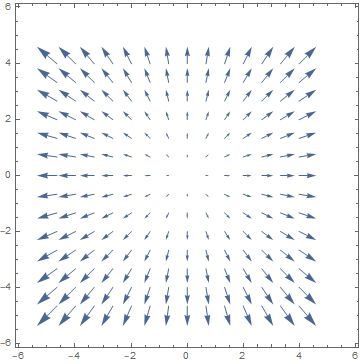
\includegraphics[scale=0.5]{plot_of_a_field.png}
        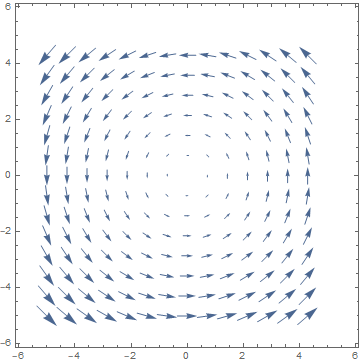
\includegraphics[scale=0.5]{plot_of_b_field.png}
        \caption{Vector fields \(\vv a = \vv r\) and \(\vv b = \vv\omega\times\vv r\) in the \(\ve 1-\ve 2\) plane}
        \label{fig:vector fields a and b}
    \end{figure}
    \subsection{Geometric Interpretation}
    The divergence at a point can be thought of as a measure of how much the flux at that points acts like a source.
    If there are more field lines coming out of that point than going in the divergence is positive.
    If more are going in than coming out then the divergence is negative.
    Finally if the same number of field lines is going in as coming out then the field has zero divergence at that point.
    A field where the divergence is zero every where is known as solenoidal.
    
    The curl at a point can be thought of as a measure of how much the field would cause a small ball at that point to rotate if the field represented the velocity of a fluid.
    The direction of the curl follows the right hand grip rule.
    In the special case where the curl is zero everywhere the field is said to be irrotational.
    
    \subsection{Laplacian}
    The Laplacian operator \(\laplacian\) can be thought of as \(\div\grad\).
    In Cartesian coordinates it is
    \begin{align*}
        \laplacian &= \div\grad\\
        &= \ve i\pdvx i\cdot \ve j\pdvx j\\
        &= \ve i\cdot\ve j\pdvx i\pdvx j\\
        &= \delta_{ij}\pdvx i\pdvx j\\
        &= \pdvx i\pdvx i\\
        &= \sum_i \pdvx i^2
    \end{align*}
    Here we have used the fact that \(\pdvx i\ve j = 0\) and the notation:
    \[\pdvx i^n = \pdv[n]{x_i}\]
    The Laplacian is a scalar operator and as such can act on either a scalar or vector field.
    If it acts on a scalar field it returns a scalar field and if it acts on a vector field it returns a vector field.
    In general if the Laplacian acts on an \(n\)-tensor field it returns an \(n\)-tensor field.
    The Laplacian can be calculated as the divergence of the gradient but it is often easier to calculate directly.
    \[\laplacian\varphi = (\grad\cdot\grad)\varphi = \div(\grad\varphi)\]
    \example
    \[\laplacian r^2 = \div(\grad r^2) = \div(2r) = 2\div r = 2\cdot 3 = 6\]
    \[\laplacian(\vv a\cdot\vv r) = \div(\grad(\vv a\cdot\vv r)) = \div\vv a = 0\]
    for constant \(\vv a\).
    
    \subsection{Vector Operator Identities}
    \subsubsection{Distributive Laws}
    \[\div(\vv a + \vv b) = \div\vv a + \div\vv b\tag{A}\]\label{eqn:A}
    This follows from the distributive property of partial derivatives:
    \[[\div(\vv a + \vv b)]_i = \pdvx i(a_i + b_i) = \pdvx i a_i + \pdvx i b_i = [\div\vv a]_i + [\div\vv b]_i\]
    \[\curl(\vv a + \vv b) = \curl\vv a + \curl\vv b\tag{B}\]
    This follows from the distributive property of partial derivatives:
    \[[\curl(\vv a + \vv b)]_i = \varepsilon_{ijk}\pdvx j(a_k + b_k) = \varepsilon_{ijk}\pdvx j a_k + \varepsilon_{ijk}\pdvx j b_k = [\curl\vv a]_i + [\curl\vv b]_i\]
    \subsubsection{Product Laws (One Vector Field)}
    \[\div(\varphi\vv a) = (\grad\varphi)\cdot\vv a + \varphi(\div\vv a) = \grad\varphi\cdot\vv a + \varphi\div\vv a\tag{C}\]
    This follows from the product law for partial derivatives:
    \[[\div\varphi\vv a]_i = \pdvx i\varphi a_i = (\pdvx i\varphi)a_i + \varphi(\pdvx i a_i) = [\grad\varphi]_ia_i + \varphi[\div\vv a]_i = [\grad\varphi\cdot\vv a]_i + [\varphi\div\vv a]_i\]
    \[\curl(\varphi\vv a) = (\grad\varphi)\times\vv a + \varphi(\curl\vv a) = \grad\varphi\times\vv a + \varphi\curl\vv a\tag{D}\]
    This follows from the product law for partial derivatives:
    \begin{align*}
        [\curl\varphi\vv a]_i &= \varepsilon_{ijk}\pdvx j\varphi a_k\\
        &= \varepsilon_{ijk}(\pdvx j\varphi)a_k + \varepsilon_{ijk}\varphi(\pdvx j a_k)\\
        &= \varepsilon_{ijk}[\grad\varphi]_j a_k + \varphi[\curl\vv a]_i\\
        &= [\grad\varphi\times\vv a]_i + [\varphi\curl\vv a]_i
    \end{align*}
    
    \section{More Identities}
    \subsection{Product Laws (Two Vector Fields)}
    \[\div(\vv a\times\vv b) = \vv b\cdot(\curl\vv a) - \vv a\cdot(\curl\vv b) \tag{E}\]
    This is easiest to prove using the index notation:
    \begin{align*}
    \div(\vv a\times\vv b) &= \varepsilon_{ijk}\pdvx i a_jb_k\\
    &= \varepsilon_{ijk}(\pdvx ia_j)b_k + \varepsilon_{ijk}a_j(\pdvx ib_k)\\
    &= b_k\varepsilon_{kij}\pdvx i a_j - a_j\varepsilon_{jik}\pdvx ib_k\\
    &= b_k(\curl \vv a)_k - a_j(\curl \vv b)_j\\
    &= \vv b\cdot(\curl\vv b) - \vv a\cdot(\curl\vv b)
    \end{align*}
    \[\curl(\vv a\times\vv b) = (\div\vv b)\vv a + (\vv b\cdot\grad)\vv a - (\div \vv a)\vv b - (\vv a\cdot\grad)\vv b\tag{F}\]
    This is easiest to prove using the vector triple product
    \[\vv a\times(\vv b \times\vv c) = (\vv a\cdot\vv c)\vv b - (\vv a\cdot\vv b)\vv c\]
    Note that since \(\grad\) doesn't commute with vector fields it is important that the vectors come after the dot products and not before.
    \begin{align*}
        \curl (\vv a\times\vv b) &= \pdvx i b_i\vv a - \pdvx i a_i\vv b\\
        &= (\pdvx ib_i)\vv a + b_i(\pdvx i\vv a) - (\pdvx ia_i)\vv b - a_i(\pdvx i\vv b)\\
        &= (\div\vv b)\vv a + (\vv b\cdot\grad)\vv a - (\div\vv a)\vv b - (\vv a\cdot\grad)\vv b
    \end{align*}
    \[\grad(\vv a\cdot\vv b) = (\vv a\cdot\div)\vv b + (\vv b\cdot\grad)\vv a + \vv a\times(\curl\vv b) + \vv b\times(\curl\vv a)\tag{G}\]
    %%%SEE TUTORIAL FOUR FOR PROOF
    
    \subsection{Identities with two \(\grad\)}
    \[\curl\grad\varphi = 0\tag{H}\]
    Consider one component of the curl of the gradient:
    \[[\curl\grad\varphi]_i = \varepsilon_{ijk}\pdvx j\pdvx k\varphi = 0\]
    This is because the partial derivatives commute (for sufficiently smooth \(\varphi\)) so we can consider them to form a symmetric 2-tensor \(t_{jk} = \pdvx j\pdvx k\).
    This means that we are then doing a contraction between a symmetric and antisymmetric tensor which is always zero.
    \[\div(\curl\vv a) = 0\tag{I}\]
    Consider one component of the divergence of the curl:
    \[[\div(\curl\vv a)]_i = \varepsilon_{ijk}\pdvx i\pdvx j a_k = 0\]
    This is zero for the same reason as above.
    \[\curl(\curl\vv a) = \grad(\div\vv a) - \laplacian \vv a\tag{J}\]
    Identities A-D and H-I should be known.
    
    We can use J to find the Laplacian in curvilinear coordinates if we already know the curl, divergence and gradient.
    
    \example
    Let \(\vv c\) be a constant vector.
    What the curl of the following vector potential?
    \[\vv A = (\vv c\times\vv r)r^{-3}\]
    \begin{align*}
        \curl \vv A &= \curl[(\vv c\times\vv r)r^{-3}]\\
        &= \grad r^{-3} \times (\vv c\times\vv r) + r^{-3}\curl(\vv c\times\vv r) &\text{Identity D}\\
        &= -3r^{-5}\vv r\times(\vv c\times\vv r) + 2r^{-3}\vv c &\grad r^n = nr^{n-2}\vv r,\;\curl(\vv c\times\vv r) = 2\vv c\\
        &= -3r^{-5}[\vv c(\vv r\cdot\vv r) - \vv r(\vv r\cdot \vv c)] + 2r^{-3}\vv c\\
        &= -3r^{-5}[r^2\vv c - (\vv r\cdot\vv c)\vv r] + 2r^{-3}\vv c\\
        &= -3r^{-3}\vv c + 3r^{-5}(\vv r\cdot\vv c)\vv r + 2r^{-3}\vv c\\
        &= 3r^{-5}(\vv r\cdot\vv c)\vv r - r^{-3}\vv c
    \end{align*}
    
    \subsection{Summary of Elementary Results}
    \(\vv a\) is a constant vector.
    \[\grad r = \vh r,\quad \grad r^n = nr^{n-2}\vv r = nr^{n-1}\vh r,\quad \div\vv r = 3,\quad \curl\vv r = 0\]
    \[\grad(\vv a\cdot\vv r) = \vv a,\quad (\vv a\cdot\grad)\vv r = \vv a\quad, \curl(\vv a\times\vv r) = 2\vv a,\quad \div(\vv a\times\vv r) = 0\]
    
    \part{Vector Integral Calculus}
    \section{One Dimensional Integrals}
    \subsection{Ordinary Integrals}
    The area under a function \(f\), defined over a domain \([a, b]\), can be split into \(n\) strips.
    The leftmost \(x\) coordinate of the \(j^\text{th}\) strip is \(x_j\).
    For each strip choose a value \(x_j^*\) such that \(x_j \le x_j^* \le x_{j + 1}\).
    We define the Riemann sum as
    \[S_n = \sum_{j=0}^{n}f(x_j^*)(x_{j + 1} - x_j)\]
    If the limit exists and is the same no matter what value of \(x_j^*\) is picked in the range then
    \[\lim_{n\to\infty} S_n = \int_a^bf(x)\,\dd x\]
    Almost all functions that we come across in physics are nicely behaved enough that it isn't a problem.
    One function that isn't is
    \[
        f(x) =
        \begin{cases}
            0 & x\in\bb Q\\
            1 & x\not\in \bb Q
        \end{cases}
    \]
    
    \subsection{Motivation}
    The work done under the influence of a force \(\vv F\) depends on the path \(C\) chosen.
    The work done \(\dd W\) in a small step \(\dd \vv r\) along that path is \(\dd W = \vv F\cdot\dd\vv r\).
    The total work done is then given by
    \[W = \int_C\vv F\cdot\dd\vv r\]
    To find what this is we need to ask several questions:
    \begin{itemize}
        \item How can we parametrise \(C\)?
        \item What is \(\dd\vv r\)?
        \item When is \(W\) path-independent?
    \end{itemize}
    
    \subsection{Parametrising A Curve}
    We will work in 2 dimensions for ease in this section although all concepts can easily be extended to 3 or more dimensions.
    In Cartesian coordinates a curve can be described as a set of points \((x_1, x_2)\).
    Since a curve is one dimensional it is possible to parametrise this curve with only one variable \(\lambda\) such that our coordinates can be written as functions of \(\lambda\) so
    \[x_1 = x_1(\lambda)\quad \&\quad x_2 = x_2(\lambda)\]
    The allows us to write the position vector in terms of \(\lambda\):
    \[\vv r(\lambda) = x_1(\lambda)\ve 1 + x_2(\lambda)\ve 2\]
    We can use the chain rule to find \(\dd\vv r\):
    \[\dd\vv r = \partial_\lambda\vv r(\lambda)\dd\lambda\]
    In components this is
    \begin{align*}
        \dd\vv r &= \ve 1\dd x_1 + \ve 2\dd x_2\\
        &= \ve 1\dd x_1(\lambda) + \ve 2\dd x_2(\lambda)\\
        &= \ve 1\partial_\lambda x_1(\lambda)\dd\lambda + \ve 2\partial_\lambda x_2(\lambda)\dd\lambda\\
        &= (\ve 1\partial_\lambda x_1 + \ve 2\partial_\lambda x_2)\dd\lambda\\
        &= \partial_\lambda\vv r\dd\lambda
    \end{align*}
    
    \example
    \[\vv a = -kx_1^3\ve 1 + kx_2^3\ve 2\]
    The path \(C\) is from \((1, 0)\) to \((0, 1)\) by the shortest path on the unit circle.
    Evaluate
    \[\int_C\vv a\cdot\dd\vv r\]
    The path \(C\) can be parametrised by
    \[x_1 = \cos\lambda,\qquad x_2 = \sin\lambda\]
    where \(\lambda\in[0,\pi/2]\).
    This allows us to write \(\vv a\) as
    \[\vv a = -k\cos^3\lambda\ve 1 + k\sin^3\lambda\ve 2\]
    We can also write \(\dd\vv r\) as
    \[\dd\vv r = -\ve 1\sin\lambda\dd\lambda + \ve 2\cos\lambda\dd\lambda\]
    This gives
    \[\vv a\cdot\dd\vv r = (\sin^4\lambda + \cos^4\lambda)\dd\lambda\]
    \[\int_c\vv a\cdot\dd\vv r = k\int_0^{\pi/2}\sin^4\lambda + \cos^4\lambda\dd\lambda = 2kI\]
    \[I = \int_0^{\pi/2}\sin^4\lambda\dd\lambda\]
    Here we have used the fact that the integral of sin or cos, to an even power, over a range \([a, a+\pi/2]\) is the same which is easily verified by looking at the graphs.
    This means that the integral of \(\sin^4\lambda + \cos^4\lambda\) is equal to two times the integral of \(\sin^4\lambda\) which is \(2I\).
    \begin{align*}
        I &= \int_0^{\pi/2}\sin^4\lambda\dd\lambda\\
        &= \int_0^{\pi/2}\sin^2\lambda(1 - \cos^2\lambda)\dd\lambda\\
        &= \underbrace{\int_0^{\pi/2}\sin^2\dd\lambda}_{\tilde I} - \underbrace{\int_0^{\pi/2}\sin^2\lambda\cos^2\lambda\dd\lambda}_{I'}
    \end{align*}
    We can use the same trick again in reverse to write that
    \[\tilde{I} = \int_0^{\pi/2}\sin^2\lambda\dd\lambda = \frac{1}{2}\int_0^{\pi/2}\sin^2 + \cos^2\dd\lambda = \int_0^{\pi/2}\dd\lambda = \frac{\pi}{4}\]
    \[I = \frac{\pi}{4} - I'\]
    The second integral, \(I'\), must be done by integration by parts.
    \[I' = \int_0^{\pi/2}\sin^2\lambda\cos^2\lambda\dd\lambda\]
    \[u = \cos \lambda \qquad\qquad v = \frac{1}{3}\sin^3\lambda\]
    \[u' = -\sin \lambda\qquad\qquad v' = \cos \lambda\sin^2 \lambda\]
    \[I' = \left[\frac{1}{3}\cos \lambda\sin^3 \lambda\right]_0^{\pi/2} + \frac{1}{3}\int_0^{\pi/2}\sin^4 \lambda\dd\lambda = 0 + \frac{I}{3}\]
    \[I = \frac{\pi}{4} - \frac{I}{3}\]
    \[\frac{4}{3}I = \frac{\pi}{4}\]
    \[I = \frac{3\pi}{16}\]
    Finally we can find the integral that we actually want:
    \[\int_C\vv a\cdot\dd\vv r = 2kI = \frac{3k\pi}{8}\]
    
    \subsection{Different Types of Line Integral}
    There are many different ways to integrate over a line.
    \(\varphi\) is a scalar field and \(\vv a\) is a vector field over a region \(R\) and \(C\) is a curve in \(R\).
    We define \(\dd\vv r\) as an infinitesimal step along \(C\).
    We define \(\dd s = \sqrt{\dd\vv r\cdot\dd\vv r}\).
    We can find various integrals along \(C\) such that we get a scalar result:
    \[\int\varphi\,\dd s, \qquad \int\vv a\cdot\dd\vv r\]
    or a vector result:
    \[\int\vv a\,\dd s, \qquad \int\varphi\,\dd\vv r, \qquad \int\vv a\times\dd\vv r\]
    
    If \(C\) is a close path (ie it starts and ends in the same place) then it is common to write the integral sign with a circle to show this, for example:
    \[\oint\vv F\cdot\dd\vv r\]
    is the work done around a closed path (zero for a conservative force).
    
    \example
    \[\vv a = (3x^2 + 6y)\ve 1 - 14yz\ve 2 + 20xz^2\ve 3\]
    Find the value of
    \[I = \int_C\vv a\cdot\dd\vv r\]
    where C is the path of straight lines connecting:
    \[(0, 0, 0)\to(1, 0, 0)\to(1, 1, 0)\to(1, 1, 1)\]
    We can split \(I\) in to three integrals:
    \[I_1 = \int_{(0, 0, 0)}^{(1, 0, 0)}\vv a\cdot\dd\vv r\biggr|_{y=z=0}\]
    \[I_2 = \int_{(1, 0, 0)}^{(1, 1, 0)}\vv a\cdot\dd\vv r\biggr|_{x=1,z=0}\]
    \[I_3 = \int_{(1, 1, 0)}^{(1, 1, 1)}\vv a\cdot\dd\vv r\biggr|_{x=y=1}\]
    Such that \(I = I_1 + I_2 + I_3\).
    It is easy to find \(\dd\vv r\) for each integral just by considering the geometry.
    For the three integrals \(\dd\vv r\) is given by \(\dd x\ve 1\), \(\dd y\ve 2\) and \(\dd z\ve 3\) in turn.
    We can then find \(\vv a\cdot\dd\vv r\) for each integral and use the conditions on which variables are constant to get
    \[I_1 = \int_0^1 3x^2\,\dd x = 1\]
    \[I_2 = \int_0^1 0\dd y = 0\]
    \[I_3 = \int_0^1 20z^2\dd z = \frac{20}{3}\]
    Finally
    \[I = 1 + 0 + \frac{20}{3} = \frac{23}{3}\]
    Now find the value of
    \[I' = \int_{C'}\vv a\cdot\dd\vv r\]
    where \(C'\) is the curve parametrised by
    \[x = \lambda,\qquad, y = \lambda^2,\qquad z = \lambda^3\]
    where \(\lambda\in[0, 1]\).
    \[\dd\vv r = \partial_\lambda\vv r\dd\lambda = \ve 1 + 2\lambda\ve 2 + 3\lambda^2\ve 3\]
    \[\vv a(\vv r(\lambda)) = 9\lambda^2\ve 1 - 14\lambda^5\ve 2 + 20\lambda^7\ve 3\]
    \[\vv a\cdot\dd\vv r = 9\lambda^2 - 28\lambda^6 + 30\lambda^9\]
    \[I' = \int_{C'}\vv a\cdot\dd\vv r = \int_0^19\lambda^2 - 28\lambda^6 + 30\lambda^9\,\dd\lambda\]
    \[= \left[3\lambda^3 - 4\lambda^7 + 6\lambda^10\right]_0^1 = 3 - 4 + 6 = 5\]
    So \(I\ne I'\).
    In general the integral along two different paths will not be equal.
    However if the integral is path--independent then the vector field is called conservative as if it where a force field the force would be conservative.
    We will see later that this occurs when the field has no curl.
    
    \section{Surface Integrals and Polar Coordinates}
    \subsection{Surface Elements}
    A surface element is defined as \(\dd\vv S = \dd S\vh n\) where \(\vh n\) is normal to the surface and \(\dd S\) is an infinitesimal with the same magnitude as the area.
    There is a choice for every surface in the direction of \(\vh n\) since the normal can point ``up" or ``down" from the surface.
    The convention is that for a closed surface always take the normal to be out of volume enclosed by the surface and for an open surface just pick a direction and be consistent.
    
    \subsection{Parametric Form}
    A surface can, since it is two dimensional, be described by only two parameters, say \(u\) and \(v\).
    This allows the position vector to be written as
    \[\vv r = \vv r(u, v) = x_1(u, v)\ve 1 + x_2(u, v)\ve 2 + x_3(u, v)\ve 3\]
    This gives line and surface elements:
    \[\dd \vv r = \partial_u\vv r\dd u + \partial_v\vv r\dd v\]
    \[\dd\vv S = \partial_u\vv r\dd u\times \partial_v\vv r\dd v\]
    since the cross product gives the normal to the surface with the magnitude of the area.
    The choice in the order in the terms in the cross product is due to the choice in orientation of the surface normal.
    The coordinates \(u\) and \(v\) are orthogonal if \(\partial_u\vv r\) and \(\partial_v\vv r\) are orthogonal.
    
    \subsection{Plane Polar Coordinates}
    Plane polar coordinates are another coordinate system to describe a point in the plane.
    Instead of giving an \(x\) and \(y\) component to each point its distance, \(\rho\), from the origin and the anticlockwise angle, \(\varphi\), from some predefined 0 is given.
    \(\rho\in[0, \infty)\) and \(\varphi\in[0, 2\pi)\).
    The Cartesian coordinates are given by
    \[x_1(\rho, \varphi) = \rho\cos\varphi,\qquad x_2(\rho, \varphi) = \rho\sin\varphi\]
    Which gives the relations
    \[\rho = \sqrt{x_1^2 + x_2^2},\qquad \tan\varphi = \frac{x_2}{x_1}\]
    A position vector with Cartesian unit vectors is
    \[\vv r = \rho\cos\varphi \ve 1 + \rho\sin\varphi \ve 2\]
    We can also find unit vectors in this new coordinate system:
    \[\ve\rho = \frac{\partial_\rho\vv r}{|\partial_\rho\vv r|} = \cos\varphi\ve 1 + \sin\varphi\ve 2 = \frac{1}{\rho}\vv r\]
    since \(|\partial_\rho\vv r| = 1\).
    \[\ve\varphi = \frac{\partial_\varphi\vv r}{|\partial_\varphi\vv r|} = -\sin\varphi\ve 1 + \cos\varphi\ve 2\]
    since\(|\partial_\varphi\vv r| = \rho\).
    We can check that these are orthonormal by computing the dot products:
    \[\ve\rho \cdot\ve\varphi = -\cos\varphi\sin\varphi + \sin\varphi\cos\varphi = 0\]
    \[\ve\rho\cdot\ve\rho = \cos^2\varphi + \sin^2\varphi = 1\]
    \[\ve\varphi\cdot\ve\varphi = \sin^2\varphi + \cos^2\varphi = 1\]
    As expected \(\ve\rho\cdot\ve\rho = \ve\varphi\cdot\ve\varphi = 1\) and \(\ve\rho\cdot\ve\varphi = 0\).
    A vector, \(\vv a\), in this orthonormal basis set, \(\{\ve\rho, \ve\varphi\}\), can be written as
    \[\vv a = a_\rho\ve\rho + a_\varphi\ve\varphi\]
    where \(a_\rho = \vv a\cdot\ve\rho\) and \(a_\varphi = \vv a\cdot\ve \varphi\).
    Note that \(\ve\rho\) and \(\ve\varphi\) are position dependent.
    A position vector in this basis is
    \[\vv r = x_\rho\ve\rho + x_\varphi\ve\varphi\]
    \[x_\varphi = \vv r\cdot \ve\varphi = \rho(\cos\varphi\ve 1 + \sin\varphi\ve 2)\cdot(-\sin\varphi\ve 1 + \cos\varphi\ve 2) = 0\]
    This makes sense as \(\vv r\) has no \(\varphi\) dependence.
    \[x_\rho = \vv r\cdot\ve\rho = \rho(\cos\varphi\ve 1 + \sin\varphi\ve 2)\cdot(\cos\varphi\ve 1 + \sin\varphi\ve 2) = \rho\]
    So a position vector can be written as
    \[\vv r = \rho\ve\rho\]
    
    \subsection{Cylindrical Coordinates}
    Cylindrical coordinates extend plane polar coordinates into the third dimension.
    They are the same as plane polar coordinates but introduce a new \(z\) component in the \(\ve 3\) direction.
    The relation of this \(z\) component to Cartesian coordinates is simply \(x_3 = z\).
    This means that \(z\in(-\infty, \infty)\) and \(\ve z = \ve 3\).
    Extending position vector into cylindrical coordinates we get
    \[\vv r = \rho\ve\rho + z\ve z\]
    \(\{\ve\rho, \ve\varphi, \ve z\}\) is an orthonormal, right handed, basis set:
    \[\ve z = \ve\rho\times\ve\varphi\]
    A vector, \(\vv a\), in this basis is given by
    \[\vv a = a_\rho\ve\rho = a_\varphi\ve\varphi + a_z\ve z\]
    where \(a_\rho = \vv a\cdot\ve\rho\), \(a_\varphi = \vv a\cdot\ve\varphi\) and \(a_z = \vv a\cdot\ve z\).
    
    \subsection{Spherical Polar Coordinates}
    Spherical coordinates are composed of a distance, \(r\), from the origin, an angle, \(\vartheta\), from the \(x_3\) axis and an angle, \(\varphi\), as in plane polar coordinates.
    The Cartesian components are given by
    \[x_1 = r\sin\vartheta\cos\varphi, \qquad x_2 = r\sin\vartheta\sin\varphi, \qquad x_3 = r\cos\vartheta\]
    \begin{multline*}
    r^2 = x_1^2 + x_2^2 + x_3^2 = r^2\sin^2\vartheta\cos^2\varphi + r^2\sin^2\vartheta\sin^2\varphi + r^2\cos^2\vartheta \\= r^2[\sin^2\vartheta(\cos^2\varphi + \sin^2\varphi) + \cos^2\vartheta] = r^2(\sin^2\vartheta + \cos^2\vartheta) = r^2
    \end{multline*}
    \[\cos\vartheta = \frac{x_3}{r},\qquad \tan\varphi = \frac{x_2}{x_1}\]
    \(r\in[0, \infty)\), \(\vartheta\in[0, \pi)\) and \(\varphi\in[0, 2\pi)\).
    The unit vectors are
    \[\ve r = \frac{\partial_r\vv r}{|\partial_r\vv r|} = \sin\vartheta\cos\varphi\ve 1 + \sin\vartheta\sin\varphi\ve 2 + \cos\vartheta\ve 3\]
    since \(|\partial_r\vv r| = 1\).
    \[\ve\vartheta = \frac{\partial_\vartheta\vv r}{|\partial_\vartheta\vv r|} = \cos\vartheta\cos\varphi\ve 1 + \cos\vartheta\sin\varphi\ve 2 + \sin\vartheta\ve 3\]
    since \(|\partial_\vartheta\vv r| = r\)
    \[\ve\varphi = \frac{\partial_\varphi\vv r}{|\partial_\varphi\vv r|} = -\sin\varphi\ve 1 + \cos\varphi\ve 2\]
    since \(|\partial_\varphi\vv r| = r\sin\vartheta\)
    
    \section{More Surface Integrals and Flux}
    \subsection{Flux}
    The flux of a vector field through a surface is a measure of how much that field flows through the surface in a direction normal to the surface.
    Let \(\vv V(\vv r)\) be a vector field.
    The flux of \(\vv V\) through a surface \(S\) with surface elements \(\dd\vv S\) is defined as
    \[I_ = \int_S\vv V\cdot\dd\vv S = \int_S V\cos\vartheta\,\dd S\]
    If the field is entirely parallel to the surface, or zero for all points on the surface, then the flux is zero.
    The magnitude of the flux is maximal when the field is normal to the surface.
    Whether the flux is positive or negative depends on the direction chosen for the surface normal.
    For a closed surface with an outwards pointing surface normal the flux being positive means that there is a net flow out of the volume and likewise a negative flux means a net flow into the volume.
    This sounds similar to the divergence's geometric definition and we shall see why when we look at the divergence theorem and the integral definition of the divergence.
    
    \example
    One common physics example of flux is for a vector field \(\vv v\) representing the velocity of a fluid the flux across a surface gives the volume of flow through that surface in one second.
    
    Another common physics example is that the flux of an electric field through a closed surface is equal to \(Q/\varepsilon_0\) where \(Q\) is the charge enclosed in the surface.
    Likewise for a magnetic field the flux through a closed surface is always zero.
    Combined these are the first two of Maxwell's equations in integral form.
    
    \example
    Let the surface \(S\) be the sphere of radius \(R\) centred on the origin.
    A point \((x_1, x_2, x_3)\) is on this sphere if and only if
    \[x_1^2 + x_2^2 + x_3^2 = R^2\]
    Let \(\vv a(\vv r) = r^{-3}\vv r\) be a vector field.
    Note that \(a = r^{-2}\) so \(\vv a\) follows an inverse square law like gravity or the Coulomb force for a point charge.
    This sphere can be parametrised using spherical coordinates.
    The position vector, \(\vv r\), is given by
    \[\vv r = r(\sin\vartheta\cos\varphi\ve 1 + \sin\vartheta\cos\varphi\ve 2 + \cos\vartheta\ve 3)\]
    \[\partial_\vartheta\vv r = r(\cos\vartheta\cos\varphi\ve 1 + \cos\vartheta\sin\varphi\ve 2 - \sin\vartheta\ve 3) = r\ve\vartheta\]
    \[\partial_\varphi\vv r = r(-\sin\vartheta\sin\varphi\ve 1 + \cos\vartheta\cos\varphi\ve 2) = r\sin\vartheta\ve\varphi\]
    The surface normal is then
    \[
        \partial_\vartheta\vv r\times\partial_\varphi\vv r = r^2
        \begin{vmatrix}
            \ve 1 & \ve 2 & \ve 3\\
            \cos\vartheta\cos\varphi & \cos\vartheta\sin\varphi & -\sin\vartheta\\
            -\sin\vartheta\sin\varphi & \cos\vartheta\cos\varphi & 0
        \end{vmatrix}
    \]
    With a lot of work this can be shown to be \(r^2\sin\vartheta\ve r\).
    It is easier to find the surface normal using spherical coordinates
    \[\partial_\vartheta\vv r\times\partial_\varphi\vv r = r\ve\vartheta\times r\sin\vartheta\ve\varphi = r^2\sin\vartheta\ve r\]
    So a surface element is
    \[\dd \vv S = (\partial_\vartheta\vv r\times\partial_\varphi\vv r)\dd\vartheta\dd\varphi = r^2\sin\vartheta\dd\varphi\dd\vartheta\ve r\]
    
    \subsection{Other Surface Integrals}
    Like with line integrals there are different ways to integrate over a surface.
    We define \(\dd S = \sqrt{\dd \vv S\cdot\dd\vv S}\).
    \(\varphi\) and \(\vv a\) are a scalar and vector field respectively over a region \(R\) and \(S\) is a surface in \(R\) the we can find various integrals over \(S\) such that we get a scalar result:
    \[\int\varphi\,\dd S,\qquad \int\vv a\cdot\dd\vv S\]
    or a vector result:
    \[\int\vv a\,\dd S,\qquad \int\varphi\,\dd\vv S,\qquad \int\vv a\times\dd\vv S\]
    
    One common integral is
    \[\int_S\dd S\]
    which gives the surface area of \(S\).
    Another useful result is that for a closed surface \(S\)
    \[\oint_S\dd\vv S = \vv 0\]
    since all of the components cancel to zero by the symmetry of the situation.
    
    \section{Volume Integrals}
    The volume integral of a scalar field \(f\) over a volume \(V\) is denoted as below and in Cartesian coordinates calculated as
    \[\int_V f(\vv r)\,\dd V = \iiint_V f(\vv r)\,\dd x\,\dd y\,\dd z\]
    Where the limits of the three integrals on the right hand side are chosen such that the entire volume is integrated over.
    Note that if \(f(\vv r) = 1\) then the integral over \(V\) gives the volume of \(V\).
    
    \example
    Integrate \(f(x, y, z) = xyz^2\) over the cube with diagonally opposite corners \((0, 0, 0)\) and \((a, b, c)\).
    \[I = \int_V f(x, y, z)\,\dd V = \int_0^c\int_0^b\int_0^a xyz^2\,\dd x\,\dd y\,\dd z = \int_0^c z^2\,\dd z\int_0^b y\,\dd y\int_0^a z\,\dd x = \left[\frac{z^3}{3}\right]_0^c\left[\frac{y^2}{2}\right]_0^b\left[\frac{x}{2}\right]_0^a = \frac{a^2b^2c^3}{12}\]
    Unfortunately not all integrals are this easily evaluated.
    Consider the octant of the unit sphere:
    \[V = \{(x, y, z)|x^2+y^2+z^2 \le 1,\; x, y, z\ge 0\}\]
    The integral over this volume of a function, \(f\), is
    \[\int_V f\,\dd V = \int_0^1\int_0^{\sqrt{1 - z^2}}\int_0^{\sqrt{1 - z^2 - y^2}}f\,\dd x\,\dd y\,\dd z\]
    Even for simple functions \(f\) the limits on the first integral makes the later integrals difficult to calculate.
    
    Many volume integrals can be simplified by parametrisation.
    This is equivalent to a change of coordinates.
    In three dimensions three parameters are needed to describe a volume.
    If a position vector can be parametrised by \(u\), \(v\) and \(w\) then \(\vv r = \vv r(u, v, w)\).
    In this case
    \[\dd\vv r = \partial_u\vv r\dd u + \partial_v\vv r\dd v + \partial_w\vv r\dd w\]
    This expands out into nine terms.
    The \(\ve i\) term is
    \[\dd\vv r\cdot\ve i = \partial_u x_i\dd u + \partial_v x_i\dd u + \partial_w x_i\dd w\]
    The volume element \(\dd V\) is given by a scalar triple product:
    \[\dd V = |(\partial_u\vv r, \partial_v\vv r, \partial_w\vv r)|\dd u\dd v\dd w\]
    This is the same as the result using the Jacobian
    \[J = |(\partial_u\vv r, \partial_v\vv r, \partial_w\vv r)| = |\det(\partial_{u_i}x_i)|\]
    where \(\vv r = x_i(u_1, u_2, u_3)\ve i\).
    
    \example
    A cylinder of height \(c\) and radius \(a\) is placed around the \(z\) axis with one face in the plane \(z = 0\).
    Find the volume of the cylinder.
    
    A volume element is given by
    \[\dd V = |\partial_\rho\vv r\cdot(\partial_\varphi\vv r\times\partial_z\vv r)|\dd\rho\dd\varphi\dd z = \rho\dd\rho\dd\varphi\dd z\]
    \[V = \int_V\dd V = \int_0^c\int_0^{2\pi}\int_0^a\rho\,\dd\rho\,\dd\varphi\dd z = \pi a^2 c\]
    which is what we would expect
    
    \example
    Find the volume of a sphere radius \(r\).
    A volume element is given by
    \[\dd V = |\partial_r\vv r\cdot(\partial_\varphi\vv r\times\partial_\vartheta\vv r)|\dd\rho\dd\vartheta\dd\varphi = r^2\sin\vartheta\dd r\dd\vartheta\dd\varphi\]
    \[V = \int_V\,\dd V = \int_0^\pi\int_0^{2\pi}\int_0^r r^2\sin\vartheta\,\dd r\,\dd\vartheta\,\dd\varphi = 2\pi[-\cos\vartheta]_0^\pi\frac{r^3}{3} = \frac{4}{3}\pi r^3\]
    
    \subsection{Integrals Over Vector Fields}
    A volume integral can also be done over a vector field \(\vv a\).
    In this case the result is an integral
    \[\vv I = \int_V\vv a\,\dd V = \ve i\iiint_V a_i\,\dd x_1\,\dd x_2\,\dd x_3\]
    So there are three integrals over the three basis vectors resulting in nine total integrals.
    
    \section{Divergence Theorem}
    \subsection{Integral Definition of Divergence}
    Let \(\vv a\) be a vector field and \(\delta V\) be a volume with boundary \(\delta S\).
    Let \(\vv P\) be a point in \(\delta V\).
    We define the divergence of \(\vv a\) at point \(\vv P\) as
    \[\divword\vv a|_{\vv P} = \lim_{\delta V\to 0}\frac{1}{\delta V} \int_{\delta S} \vv a\cdot\dd\vv S\]
    It can be shown that this is independent of the shape chosen for \(\delta V\).
    We will show that this is the same as the definition of \(\div\vv a\) in Cartesian coordinates which will show that they are the same operator.
    
    \subsection{Showing Equivalence}
    Since we can choose any shape for \(\delta V\) we pick a cube with diagonally opposite vertices at \((0, 0, 0)\) and \((\delta_x, \delta_y, \delta_z)\).
    The point \(\vv P = (x_0, y_0, z_0)\) is at the centre of the cube so \(\vv P = (\delta_x/2, \delta_y/2, \delta_z/2)\).
    We will start by considering the flux across the planes normal to \(\ve 1\).
    A surface element on these planes is given by \(\dd\vv S_x = \pm\dd y\dd z\ve 1\) where the \(\pm\) comes from the two faces with surface normals antiparallel.
    This gives \(\vv a\cdot\dd\vv S_x = \pm a_x\dd y\dd z\).
    We now compute the right hand side of the divergence definition:
    \[\frac{1}{\delta V}\int_{\delta S_x}\vv a\cdot\dd\vv S = \frac{1}{\delta V}\iint\dd z\,\dd y\left[a_x\left(x_0 + \frac{\delta_x}{2}, y, z\right) - a_x\left(x_0 - \frac{\delta_x}{2}, y, z\right)\right]\]
    Where the two \(a_x\) terms are due to the two faces.
    We can make \(\delta V\to 0\) by taking \(\delta_x, \delta_y, \delta_z\to 0\).
    Since \(\delta_x\) is small we can Taylor expand this to get
    \[\frac{1}{\delta V}\iint\dd y\,\dd x \left[a_x(x_0, y_0, z_0) + \frac{\delta_x}{2}\partial_x a_x|_{(x_0, y, z)} + \mathcal{O}(\delta_x^2) - \left(a_x(x_0, y_0, z_0) - \frac{\delta_x}{2}\partial_x a_x|_{(x_0, y, z)} + \mathcal{O}(\delta_x^2)\right)\right]\]
    Cancelling terms we get
    \[\frac{\delta_x}{\delta V}\iint\dd y\,\dd z\partial_xa_x\]
    We can use the fact that as \(a\to b\)
    \[\int_a^b f(x)\,\dd x \to f(x_0)(a - b)\]
    for \(x_0\in[a, b]\), to find the value of this double integral since both integrals are over vanishing ranges \(\delta_y, \delta_z\to 0\)
    \[\frac{\delta_x}{\delta V}\iint\dd y\,\dd z\partial_x a_x = \frac{\delta_x\delta_y\delta_z}{\delta V}\partial_x a_x = \partial_x a_x|_{(x_0, y_0, z_0)}\]
    since \(\delta V = \delta_x\delta_y\delta_z\).
    Doing the same for the other four faces of the cube we see that
    \[\divword \vv a = \partial_x a_x + \partial_y a_y + \partial_z a_z\]
    which is the same as the definition of \(\div\vv a\) in Cartesian coordinates.
    
    \subsection{Intuitive Understanding of Divergence}
    This allows us get a better intuitive understanding of divergence as a measure of the flux out of a point.
    For a vector field, \(\vv a\), if \(\div\vv a > 0\) then there must be a net flux out of the point, if \(\div\vv a < 0\) then there must be a net flux into the point.
    This makes these two points a source and a sink respectively.
    If \(\div\vv a = 0\) then \(\vv a\) must be constant at the point so the flux in is equal to the flux out.
    This agrees with the Cartesian definition where \(\div\vv a\) is a derivative of \(\vv a\) so if \(\vv a\) is constant then this will be zero.
    
    \subsection{The Divergence Theorem}
    Let \(\vv a\) be a vector field and \(V\) be a volume with surface \(S\) (sometimes, confusingly, called \(\delta V\)).
    The divergence theorem is
    \[\int_V\div\vv a\,\dd V = \int_S\vv a\cdot\dd\vv S\]
    This is a generalisation to three dimensions of the fundamental theorem of calculus:
    \[\int_a^b\partial_xf(x)\,\dd x = f(b) - f(a)\]
    
    We consider an arbitrary volume \(V\).
    This volume can be approximated using small cubes.
    The \(i^\text{th}\) cube has a volume \(\delta V^{(i)}\) and surface \(\delta S^{(i)}\).
    It is at position \(\vv r^{(i)}\).
    The divergence at this cube can be calculated as
    \[\div\vv a(\vv r^{(i)}) = \frac{1}{\delta V^{(i)}} \int_{\delta S^{(i)}}\vv a\cdot\dd\vv S + \varepsilon^{(i)}\]
    where \(\varepsilon^{(i)}\) is a correction term to account for the fact that \(\delta V^{(i)}\) is finite.
    We can then approximate the integral of the divergence as the sum of this over all cubes.
    Let \(N\) be the number of cubes, then
    \[\sum_{i = 1}^N \div\vv a(\vv r^{(i)})\delta V^{(i)} = \sum_{i = 1}^N \int_{\delta S^{(i)}}\vv a\cdot\dd\vv S + \varepsilon^{(i)}\delta V^{(i)}\]
    Consider the adjacent cubes 1 and 2 with volumes \(\delta V^(1)\) and \(\delta V^{(2)}\) respectively.
    Define the total volume of both as \(\delta V^{(1\cup2)}\).
    The surface area of this volume is then given by the surface areas of the two cubes minus two times the area that they share.
    We will denote this \(\delta S^{(1\oplus 2)}\).
    Fortunately since both surfaces have equal and opposite surface normals at the intersection of the two surfaces the contribution of this cancels in the sum.
    This means
    \[\int_{\delta S^{(1)}}\vv a\cdot\dd\vv S + \int_{\delta S^{(2)}}\vv a\cdot\dd\vv S = \int_{\delta S^{(1\oplus 2)}}\vv a\cdot\dd\vv S\]
    We now let \(N\to\infty\) and hence \(\delta V^{(i)}\to 0\).
    \[\sum_{i = 1}^N\div\vv a(\vv r^{(i)})\delta V^{(i)} \to \int_V\div\vv a\,\dd V\]
    \[\sum_{i = 1}^N\epsilon^{(i)}\delta V^{(i)} \to 0\]
    assuming that \(\varepsilon < 1/N\) so shrinks faster than \(N\) grows.
    \[\sum_{i = 1}^N\int_{\delta S^{(i)}}\vv a\cdot\dd\vv S \to\int_S\vv a\cdot\dd\vv S\]
    From this we get
    \[\int_V\div\vv a\,\dd V = \int_S\vv a\cdot\dd\vv S\]
    which is the divergence theorem.
    
    \subsection{Volume of a Body Using the Divergence Theorem}
    Recall that \(\div\vv r = 3\) and that the volume integral of one is the volume.
    This means that
    \[\frac{1}{3}\int_V\div\vv r\,\dd V = \frac{1}{3}\int_V 3\,\dd V = \int_V\dd V = V\]
    
    \example
    Use this to find the volume of the upper hemisphere with radius \(R\).
    We define a coordinate system with the origin at the centre of the flat circular base of the hemisphere which is in the \(x_1{-}x_2\) plane where \(x_3 = 0\).
    We consider two surfaces \(S_c\) and \(S_b\) where \(S_c\) is the curved surface and \(S_b\) is the base.
    The whole surface is \(S = S_c + S_b\).
    A surface element of the base is given by \(\dd\vv S_b = -\ve 3\dd S_b\) hence \(\vv r\cdot\dd\vv S_b = -x_3\) but \(x_3 = 0\) so \(\vv r\cdot\dd\vv S_b = 0\).
    A surface element of the curved surface is given in spherical coordinates by
    \[\dd\vv S_c = R^2\sin\vartheta\dd\vartheta\dd\varphi\ve r\]
    so \(\vv r\cdot\dd\vv S_c = R\ve r\cdot R^2\sin\vartheta\dd\vartheta\dd\varphi\ve r =R^3\sin\vartheta\dd\vartheta\dd\varphi\).
    Hence the volume of the hemisphere is
    \[V = \frac{1}{3}\int_V\div\vv r\,\dd V = \int_S\vv r\cdot\dd\vv S = \int_{S_b}\vv r\cdot\dd\vv S_b + \int_{S_c}\vv r\cdot\dd\vv S_c = \frac{R^3}{3}\int_0^{2\pi}\dd\varphi\int_0^{\pi/2}\sin\vartheta\,\dd\vartheta\]
    \[V = \frac{2}{3}\pi R^3[-\cos\vartheta]_0^{\pi/2} = \frac{2}{3}\pi R^3\]
    which is half the volume of a sphere as we would expect.
    
    \section{Continuity Equation and Gauss's Law}
    \subsection{Continuity Equation}
    A volume \(V\) contains a fluid of density \(\rho(\vv r, t)\).
    The fluid has velocity \(\vv v(\vv r)\).
    The flux per unit time of mass is the loss of mass in volume \(V\) per unit time and is given by
    \[\int_S\rho\vv v\cdot\dd\vv S\]
    where \(S\) is the surface of \(V\).
    \(\rho\vv v = \vv J\) is a current density.
    The loss of mass per unit time can also be calculated as
    \[-\partial_t\int_V\rho\,\dd V\]
    since the volume integral of a density is the mass and the \(-\partial_t\) gives the rate of decrease.
    Hence
    \[\int\rho\vv v\cdot\dd\vv S = -\partial_t\int_V\rho\,\dd V\]
    By the divergence theorem
    \[\int_V\div(\rho\vv v)\,\dd V = -\partial_t\int_V\rho\,\dd V\]
    for a time independent volume this is
    \[\int_V\div(\rho\vv v)\,\dd V = \int_V-\partial_t\rho\,\dd V\]
    For this to be true for arbitrary volume \(V\) it is necessary and sufficient that the integrands be equal
    \[\div(\rho\vv v) = -\partial_t\rho\]
    Hence
    \[\partial_t\rho + \div(\rho\vv v) = \partial_t\rho + \div\vv J = 0\]
    This same analysis works for other context for example:
    \begin{itemize}
        \item \(\rho\) is thermal energy and \(\vv J\) is heat current density
        \item \(\rho\) is electric charge density and \(\vv J\) is electric current density
        \item \(\rho\) is a quantum mechanical probability density and \(\vv J\) is a probability current density
    \end{itemize}
    There are some special cases:
    \begin{itemize}
        \item Mass flux conservation: \(\partial_t\rho = \div\vv J = 0\).
        No net flux means the mass in the volume is constant
        \item Incompressible fluid: \(\partial_t\rho = 0,\), \(\pdvx i\rho = 0 \implies \div\vv J = \rho\div\vv v = 0\).
        No local change in fluid density means the fluid is incompressible and hence \(\rho\) is a constant.
    \end{itemize}
    
    \subsection{Sources and Sinks}
    The amount to which a certain volume, \(V\), with surface \(S\) is a source of a vector field \(\vv a\) is characterised by
    \[x_s = \int_S \vv a\cdot\dd\vv S\]
    if \(x_s > 0\) then the volume is a net source of \(\vv a\),
    if \(x_s < 0\) then the volume is a net sink of \(\vv a\) and if \(x_s = 0\) then the volume is neither a source nor sink of \(\vv a\).
    This idea can be localised using the integral definition of the divergence.
    \[\div\vv a|_{\vv P} = \lim_{V\to 0}\frac{1}{V}\int_S\vv a\cdot\dd\vv S\]
    this gives a measure of how the point \(\vv P\) acts as a source or sink with the same sign requirements as the global version.
    
    \subsection{Electrostatics}
    The electric field from a points charge at the origin is
    \[\vv E(\vv r) = \frac{q}{4\pi\varepsilon_0}\frac{1}{r^3}\vv r\]
    This has a \(r^{-2}\) characteristic and we have already shown that for \(r \ne 0\) this gives a divergence of
    \[\div\vv E = \frac{q}{4\pi\varepsilon_0}\div(r^{-3}\vv r) = \frac{q}{4pi\varepsilon_0}\left[\grad r^{-3}\cdot\vv r + r^{-3}\div\vv r\right] = 0\]
    Formally if we want to include the point \(r = 0\) then we get
    \[\div(r^{-3}\vv r) = 4\pi\delta^{(3)}(\vv r)\]
    where \(\delta^{(3)}\) is the three dimensional Dirac delta function.
    Let \(S\) be a sphere of radius \(R\) centred at the origin.
    Then \(\dd\vv S = \ve r r^2\dd\vartheta\dd\varphi\)
    \[\int_S\vv E\cdot\dd\vv S = \frac{q}{4\pi\varepsilon_0}\int_S\frac{\vv r\cdot\dd\vv S}{r^3} = \frac{q}{4\pi\varepsilon_0}\int_0^{2\pi}\int_0^{\pi}\frac{\vv r\cdot\ve r}{r^3}r^2\sin\vartheta\,\dd\vartheta\,\dd\varphi = \frac{q}{4\pi\varepsilon_0}2\pi[-\cos]_0^{\pi} = \frac{q}{\varepsilon_0}\]
    This also holds for a charge enclosed by \(S\) but not at the origin.
    We want to show that it holds for an arbitrary surface.
    
    Suppose \(S\) is a surface containing a point charge.
    We remove a small sphere, \(S_1\) around the point charge so that it is not in the surface \(S\).
    The normal vectors for this sphere point into the sphere as they point out of \(S\).
    Everywhere in \(S\) but not \(S_1\) the divergence is zero.
    Thus the flux across the surfaces \(S\) and \(S_1\) (ie the new surface with the sphere removed) is
    \[\int_{S+S_1} \vv E\cdot\dd\vv S = \int_{V - V_1}\div\vv E\,\dd V = \int_{V-V_1}0\,\dd V = 0\]
    where the first equality is by the divergence theorem and \(V - V_1\) is the volume contained by \(S\) minus the volume contained by \(S_1\).
    The flux can also be calculated as
    \[\int_{S+S_1}\vv E\cdot\dd\vv S = \int_S\vv E\cdot\dd\vv S + \int_{S_1}\vv E\cdot\dd\vv S = \int_S\vv e\cdot\dd\vv S - \frac{q}{\varepsilon_0} = 0\]
    \[\implies \int_S\vv E\cdot\dd\vv S = \frac{q}{\varepsilon_0}\]
    note the negative sign because of the inwards pointing surface vectors.
    From this we can see that this holds for any surface.
    
    For \(N\) charges, \(q_i\), we do the same but cut out \(N\) spheres \(S_i\).
    We apply the same logic and the empirical result that electric fields add linearly and we get
    \[\int_S\vv E\cdot\dd\vv S = \int_S\sum_{i = 1}^N\vv E_i\cdot\dd\vv S = \sum_{i = 1}^N\int_{S_i}\vv E_i\cdot\dd\vv S = \sum_{i = 1}^N\frac{q_i}{\varepsilon_0} = \frac{Q_\text{total}}{\varepsilon_0}\]
    where \(Q_\text{total}\) is the total charge contained by the surface.
    This also generalises to charge density distributions \(\rho(\vv r)\) defined such that
    \[\int\rho(\vv r)\,\dd V = Q_\text{total}\]
    in this case we get
    \[\int_S\vv E\cdot\dd\vv S = \frac{1}{\varepsilon_0}\int\rho(\vv r)\,dd V = \frac{Q_\text{total}}{\varepsilon_0}\]
    This is Gauss's law and is the first of Maxwell's laws.
    This is it in integral form, we can get it in differential form using the divergence theorem:
    \[\int_S\vv E\cdot\dd\vv S = \int_V\div\vv E\,\dd V = \frac{1}{\varepsilon_0}\int\rho(\vv r)\,\dd V\]
    For this to be true for arbitrary volumes, \(V\), it is necessary and sufficient for the integrands to be equal
    \[\div\vv E = \frac{\rho}{\varepsilon_0}\]
    This is Gauss's law in differential form.
    
    \subsection{Corollaries of the Divergence Theorem}
    If the vector field \(\vv a\) is a constant then \(\div\vv a = 0\) so by the divergence theorem
    \[0 = \int_V\div\vv a = \oint_S\vv a\cdot\dd\vv S = \vv a\cdot\oint\dd\vv S = 0\]
    For this to be true for arbitrary constant \(\vv a\) then
    \[\oint_S\dd\vv S = \vv 0\]
    that is that the vector integral over any closed surface is zero.
    It has to be closed as the divergence theorem takes \(S\) as the surface containing \(V\) which must mean that \(S\) is closed.
    
    If instead \(\vv a = p(\vv r)\vv c\) for some constant vector \(\vv c\) then
    \[\div\vv a = \div(p\vv c) = \grad p\cdot\vv c + p\div\vv c = \grad p\cdot\vv c\]
    since the divergence of a constant vector is zero.
    From this and the divergence theorem we get
    \[\vv c\cdot\int_V\grad p\,\dd V = \int_V\vv c\cdot\grad p\,\dd V = \int_V\div\vv a\,\dd V = \int_S\vv a\cdot\dd\vv S = \int_Sp\vv c\cdot\dd\vv S = \vv c\cdot\int_S p\,\dd\vv S\]
    for this to be true for arbitrary constants \(\vv c\) we require
    \[\int\grad p\,\dd V = \int p\,\dd\vv S\]
    
    If \(\vv a(\vv r) = \vv b(\vv r)\times \vv c\) for some vector field \(\vv b(\vv r)\) and constant vector \(\vv c\) then
    \[\div \vv a = \vv c\cdot\curl\vv b - \vv b\cdot\curl\vv c = \vv c\cdot\curl\vv b\]
    since the curl of a constant vector is zero.
    \[\int_V\div\vv a\,\dd V = \vv c\cdot\int_V\curl\vv b\,\dd V = \int_S(\vv b\times\vv c)\cdot\dd\vv S = -\vv c\cdot\int_S\vv b\times\dd\vv S\]
    For this to hold for all \(\vv c\) we require
    \[\int_V\curl\vv b\,\dd V = -\int_S\vv b\times\dd\vv S\]
    
    \section{Stokes' Theorem}
    \subsection{Integral Definition of Curl}
    Let \(\delta C\) be a closed curve enclosing surface \(\delta S\).
    The curl of a vector field \(\vv a\) through the surface satisfies
    \[\curlword(\vv a)\cdot\vh n = \lim_{\delta S\to 0}\frac{1}{\delta S}\oint_{\delta C}\vv a\cdot\dd\vv r\]
    where \(\vh n\) is the surface normal to \(\delta S\).
    This can be used to define curl.
    Note that the directions of \(\delta C\) and \(\vh n\) are important.
    By convention we choose them to be right handed so that if your right thumb points in the \(\vh n\) direction then your fist curls in the direction of \(\delta C\).
    It can be shown that \(\curlword(\vv a)\cdot\vh n\) is independent of the shape of \(\delta C\).
    We want to show that \((\curl\vv a)\cdot\vh n = \curlword(\vv a)\cdot\vh n\).
    
    \subsection{Showing Equivalence}
    Since the curl is independent of the shape of \(\delta C\) we can choose any shape so we choose a square.
    We start with a rectangle in the \(x\)-\(y\) plane.
    The rectangle has sides \(\delta x\) and \(\delta y\) in the \(x\) and \(y\) directions respectively.
    We choose to find the curl at a point \(P = (x_0, y_0, z_0) = (\delta x/2, \delta y/2, 0)\) which is in the middle of the rectangle.
    The path along which we integrate is then from \(A\) to \(B\) to \(C\) to \(D\) and back to \(A\) where
    \[A = (\delta x, 0, 0),\qquad B = (\delta x, \delta y, 0),\qquad C = (0, \delta y, 0),\qquad D = (0, 0, 0)\]
    The surface bounded by this path is \(\delta S = \delta x\delta y\).
    The surface normal is \(\vh n = \ve 3\).
    First we compute the right hand side of the integral definition of curl.
    We get
    \begin{align*}
    \int_{\delta C}\vv a\cdot\dd\vv r &= \int_A^B\vv a\cdot\dd\vv r + \int_C^D\vv a\cdot\dd\vv r + \int_B^C\vv a\cdot\dd\vv r + \int_D^A\vv a\cdot\dd\vv r\\
    &= \int_A^B\vv a\cdot\dd\vv r - \int_D^C\vv a\cdot\dd\vv r - \int_C^B\vv a\cdot\dd\vv r + \int_D^A\vv a\cdot\dd\vv r\\
    \intertext{For the first two integrals \(\dd\vv r = \ve 2\dd y\) and for the second two \(\dd\vv r = \ve 1\dd x\)}
    &= \int_A^B a_y\,\dd x - \int_D^C a_y\,\dd y + \int_D^A a_x\,\dd x - \int_C^B a_x\,\dd x\\
    \end{align*}
    We call these integrals \(I_3\), \(I_4\), \(I_1\) and \(I_2\) respectively.
    First we consider \(I_1\).
    \[I_1 = \int_A^B a_x\,\dd x = \int_{x_-}^{x_+} a_x\left(x, y_0 - \frac{\delta y}{2}, z_0\right)\,\dd x\]
    where \(x_{\pm} = x_0\pm \delta x/2\).
    We Taylor expand this to get
    \[I_1 = \int_{x_-}^{x_+} a_x(x, y_0, z_0) - \partial_y a_x(x, y_0, z_0)\frac{\delta y}{2} + \mathcal{O}(\delta y^2)\,\dd x\]
    we can also Taylor expand \(I_2\) and we get
    \[I_2 = -\int_{x_-}^{x_+} a_x(x, y_0, z_0) + \partial_y a_x(x, y_0, z_0)\frac{\delta y}{2} + \mathcal{O}(\delta y^2)\,\dd x\]
    In anticipation of our goal of showing equivalence we will calculate \((I_1 + I_2)/\delta S\):
    \begin{align*}
    \frac{I_1 + I_2}{\delta S} &= \frac{1}{\delta x\delta y}\int_{x_-}^{x_+}-\partial a_x(x, y_0, z_0)\delta y + \mathcal{O}(\delta y^2)\,\dd x\\
    &= \frac{1}{\delta x}\int_{x_-}^{x_+}-\partial a_x(x, y_0, z_0) + \mathcal{O}(\delta y)\,\dd x
    \end{align*}
    Recall that for \(x^*\in[a, b]\) as \(a\to b\)
    \[\lim_{a\to b}\int_a^b f(x)\,\dd x = f(x^*)(b - a)\]
    so as \(\delta x\to 0\) and \(x_-\to x_+\) we get
    \[\frac{I_1 + I_2}{\delta S} = -\partial_y a_x(x_0, y_0, z_0)\]
    Similarly we can show
    \[\frac{I_3 + I_4}{\delta S} = -\partial_x a_y(x_0, y_0, z_0)\]
    Finally we get
    \[\curlword(\vv a)\cdot\ve 3 = (\partial_x a_y - \partial_y a_x)|_{(x_0, y_0, z_0)}\]
    which agrees with \(\curl\vv a|_{(x_0, y_0, z_0)}\cdot\ve 3\).
    By symmetry this argument must hold for all other orientations of the initial surface so we can say that
    \[\curlword(\vv a)\cdot\vh n = (\curl\vv a)\cdot\vh n\]
    hence the two definitions of curl are equivalent.
    
    \subsection{Intuitive Understanding of Curl}
    This gives us an intuitive understanding of curl as how much the field is in the same direction as \(\delta C\).
    The more the directions agree the more positive the curl and if they are mostly in opposite directions then the curl will be negative.
    If either there happens to be cancellation around \(\delta C\) or if the vector field is perpendicular to \(\delta C\) all around then the curl will be 0.
    
    \subsection{Stokes' Theorem}
    Stokes' theorem is
    \[\int_S (\curl\vv a)\cdot\dd\vv S = \int_C\vv a\cdot\dd\vv r\]
    This follows from the integral definition of curl.
    Consider a surface \(\delta S\), it can be approximated as being made of small squares.
    When two of these squares share an edge \(\delta C\) for each square is in opposite directions along the shared edge so the component of curl from the shared edge cancels to zero.
    This means that the curl of a vector field over the surface is the same as the sum of the curl of the vector field over each square.
    For small, but not infinitesimal squares at positions \(\vv r^{(i)}\)
    \[\curl\vv a(\vv r^{(i)})\cdot\vh n^{(i)} = \frac{1}{\delta S^{(i)}}\oint_{\delta C^{(i)}}\vv a\cdot\dd\vv r + \varepsilon^{(i)}\]
    where \(\varepsilon^{(i)}\) is an error term that goes to zero as the number of squares goes to infinity
    Multiplying through by \(\delta S\) and summing over all the squares we get
    \[\sum_{i = 1}^N \curl\vv a(\vv r^{(i)})\cdot\vh n^{(i)}\delta S^{(i)} = \sum_{i = 1}^N \oint_{\delta S^{(i)}}\vv a\cdot\dd\vv r\delta S^{(i)} + \sum_{i = 1}^N \delta S^{(i)}\varepsilon^{(i)}\]
    The second term goes to zero as \(N\) goes to infinity and the term on the left becomes an integral with \(\vh n\delta S = \delta\vv S \to \dd\vv S\), for this to always be true we require
    \[\int_S (\curl\vv a)\cdot\dd\vv S = \int_C\vv a\cdot\dd\vv r\]
    which is Stokes' theorem.
    
    \section{Stokes' Theorem In Use}
    Stokes' Theorem is a generalisation to three dimensions of
    \[\int_y \partial_x f(x)\,\dd x = f(y) + C\]
    \example
    Verify Stokes' theorem for a hemisphere of radius \(R\) and the vector field \(\vv a = 4y\ve 1 + x\ve 2 + 2z\ve 3\).
    \[\curl\vv a = -3\ve 3\]
    \[\dd\vv S = R^2\sin\vartheta\dd\vartheta\dd\varphi\ve r\]
    The left hand side of Stokes' theorem evaluates to
    \begin{align*}
        \int (\curl\vv a)\cdot\dd\vv S &= -3R^2\int_0^{\pi/2}\dd\vartheta\int_0^{2\pi}\dd\varphi\sin\vartheta\ve r\cdot\ve 3\\
        \intertext{\(\ve r\cdot\ve 3 = \cos\vartheta\)}
        &= -3R^2(2\pi)\int_0^1\dd(\cos\vartheta) \cos\vartheta\\
        &= -6\pi R^2\int_0^1\cos\vartheta\dd(\cos\vartheta)\\
        &= -6\pi R^2\frac{1}{2}\\
        &= -3\pi R^2
    \end{align*}
    Parametrising in terms of \(\varphi\) we get \(x(\varphi) = R\cos\varphi\), \(y(\varphi) = R\sin\varphi\) and \(z(\varphi) = 0\) which gives \(\vv r(\varphi) = R(\cos\varphi\ve 1 + \sin\varphi\ve 2)\).
    \[\dd\vv r = \partial_\varphi\dd\varphi = R(-\sin\varphi\ve 1 + \cos\varphi\ve 2)\dd\varphi\]
    \[\vv a\cdot\dd\vv r = R(-\sin\varphi 4y + \cos\varphi x)\dd\varphi = R^2(-4\sin^2\varphi + \cos^2\varphi)\dd\varphi\]
    The right hand side of Stokes' theorem evaluates to
    \begin{align*}
        \int_{\delta S}\vv a\cdot\dd\vv r &= R^2\int_0^{2\pi}-4\sin^2\varphi + \cos^2\varphi\,\dd\varphi\\
        &= \pi R^2(-4 + 1)\\
        &= -3\pi R^2
    \end{align*}
    which is the same as the left hand side so Stokes' theorem held.
    
    \subsection{Planar Areas as a Special Case}
    Consider the vector field 
    \[\vv a = \frac{1}{2}(-y\ve 1 + x\vee 2)\]
    The curl of this vector field is \(\curl\vv a = \ve 3\) and \(\dd\vv S = \ve 3\dd S\).
    The left hand side of Stokes' theorem is
    \[\int_S(\curl\vv a)\cdot\dd\vv S = \int_S\ve 3\cdot\dd\vv S = \int\dd S = S\]
    \[\vv a\cdot\dd\vv r = \frac{1}{2}(-y\ve 1 + x\ve 2)\cdot(\dd x\ve 1 + \dd y\ve 2) = \frac{1}{2}(x\dd y - y\dd x)\]
    The right hand side of Stokes' theorem is
    \begin{equation}\label{eqn:Green's theorem}
    S = \int_C\vv a\cdot\dd\vv r = \frac{1}{2}\oint_Cx\,\dd y - y\,\dd x
    \end{equation}
    
    \example
    Consider the curve \(x^{2/3} + y^{2/3 = 1}\).
    This can be parametrised by \(x = \cos^3\varphi\) and \(y = \sin^3\varphi\) for \(\varphi\in[0, 2\pi]\).
    \[\dd x = \partial_\varphi x\dd\varphi = -3\cos^2\varphi\sin\varphi\dd\varphi,\qquad \dd y = \partial_\varphi y\dd\varphi = 3\sin^2\varphi\cos\varphi\dd\varphi\]
    By equation \ref{eqn:Green's theorem} this gives
    \begin{align*}
        S &= \frac{1}{2}\int_0^\pi 3(\cos^4\varphi\sin^2\varphi + \sin^4\varphi\cos^2\varphi)\,\dd\varphi\\
        &= \frac{3}{2}\int_0^\pi \cos^2\varphi\sin^2\varphi\,\dd\varphi\\
        &= \frac{3}{8}\int_0^\pi \sin^22\varphi\,\dd\varphi\\
        &= \frac{3\pi}{8}
    \end{align*}
    
    \subsection{Corollaries of Stokes' Theorem}
    For a constant vector field \(\vv c\)
    \begin{enumerate}
        \item For the case where the vector field \(\vv a = \vv c\) we have \(\curl\vv a = 0\) so
        \[\oint_C\vv a\cdot\dd\vv r = \vv c\cdot\oint_C\dd\vv r = \int_S(\curl\vv a)\cdot\dd\vv r = 0 \iff \oint\dd\vv r = 0\]
        \item For a vector field \(\vv a = -Y(x, y)\ve 1 + X(x, y)\ve 2\) we have \(\curl\vv a = (\partial_x X + \partial_y Y)\ve 3\).
        Also \(\dd\vv S = \dd x\dd y\ve 3\) so
        \[(\curl\vv a)\cdot\dd\vv S = (\partial_x X + \partial_y Y)\dd x\dd y\]
        \[\dd\vv r = \dd x\ve 1 + \dd y\ve 2 \implies \vv a\cdot\dd\vv r = -Y\dd x + X\dd y\]
        \[\int_S(\partial_x X + \partial_y Y)\,\dd x\,\dd y = \int_C X\,\dd y - Y\,\dd x\]
        This is Green's Theorem
        \item For the case where the vector field is \(\vv a = \varphi(\vv r)\vv c\) then
        \[\curl\vv a = \grad\varphi\times\vv c + \varphi\curl\vv c = \grad\varphi\times\vv c\]
        since the curl of a constant is zero.
        Hence
        \[\int_S(\curl\vv a)\cdot\dd\vv S = \int_S (\grad\varphi\times\vv c)\cdot\dd\vv S = \vv c\cdot\int_S\dd\vv S\times\grad\varphi = \vv c\cdot\oint_C\varphi\,\dd\vv r\]
        To be true for all \(\vv c\) we require
        \[\oint_{\partial S} \varphi\,\dd\vv r = -\int_S\grad\varphi\times\dd\vv S\]
        Note that the case where \(\varphi = 1\) is the first item in this list.
    \end{enumerate}
    
    \subsection{Divergence and Stokes' Theorems Synopsis}
    Let \(S\) be a closed surface containing volume \(V\).
    We can consider this to be an open surface with small hole with boundary \(C\) and then let \(C\to 0\) so the surface becomes closed and also \(\int(\curl\vv a)\cdot\dd\vv S\to 0\) then
    \[\int_C\vv a\cdot\dd\vv r = \int_S(\curl\vv a)\cdot\dd\vv S = \int_V\div(\curl\vv a)\,\dd V = 0\]
    Where the first equality is by Stokes' theorem and the second by the divergence theorem and the final equality is true as the integrand is zero since the divergence of the curl is always zero.
    
    \section{Potentials}
    \subsection{Maxwell's Equations}
    One very common use of vector calculus is in Maxwell's equations.
    For electric field, \(\vv E\), magnetic field, \(\vv B\), charge density, \(\rho\), and current density, \(\vv J\), Maxwell's equations in a vacuum are
    \begin{align*}
    \div\vv E = \frac{\rho}{\varepsilon_0},&\qquad \div\vv B = 0\\
    \curl\vv E + \partial_t\vv B = 0,&\qquad \curl\vv B - \frac{1}{c^2}\partial_t\vv E = \mu_0\vv J
    \end{align*}
    It can be shown that it is always possible to write the magnetic and electric fields in terms of a vector potential, \(\vv A\), and scalar potential, \(\varphi\), such that
    \[\vv B = \curl\vv A,\qquad \vv E = -\grad\varphi + \partial_t\vv A\]
    Maxwell's equations can also been written relativistically.
    For this we work in natural units where \(c = 1\) and \(\mu_0 = 1\).
    In dot products we replace the Kronecker delta, \(\delta_{ij}\), with the Minkowski metric, \(\eta_{\mu\nu} = \mathop{\mathrm{diag}}(1, -1, -1, -1)\) where we use the sign convention \((\begin{smallmatrix} + & - & - & - \end{smallmatrix})\).
    To write Maxwell's equations we need some 4-vectors:
    \begin{itemize}
    \item The four momentum which is \(p_\mu = (E, \vv p)\) where \(E\) is the energy and \(\vv p\) is the 3-momentum.
    \item The four position which is \(x_\mu = (t, -\vv x)\) where \(t\) is the time and \(\vv x\) is the 3-position.
    \item The four potential which is \(A_\mu = (\varphi, \vv A)\) where \(\varphi\) is the scalar potential and \(\vv A\) is the 3-potential.
    \item The four current density which is \(j_\mu = (\rho, \vv j)\) where \(\rho\) is the charge density and \(\vv j\) is the 3-current density.
    \end{itemize}
    The electric and magnetic fields are combined in the electromagnetic field tensor:
    \[
        F_{\mu\nu} = \partial_\mu A_\nu - \partial_\nu A_\mu = 
        \begin{pmatrix}
            0 & E_x & E_y & E_z\\
            -E_x & 0 & -B_z & B_y\\
            -E_y & B_z& 0 & -B_x\\
            -E_z & -B_y & B_x & 0
        \end{pmatrix}
    \]
    where \(\partial_\mu\) is the covariant 4-gradient, \((\partial_t, \grad)\).
    Finally we need to define the Hodge dual which is
    \[\tilde{F}_{\mu\nu} = \frac{1}{2}\varepsilon_{\mu\nu\rho\sigma}F^{\mu\nu}\]
    where \(F^{\mu\nu} = \eta^{\mu\alpha}F_{\alpha\beta}\eta^{\beta\nu}\) and \(\eta^{\mu\nu} = \eta_{\mu\nu}\).
    This allows us to compactly write Maxwell's equations as
    \[\partial^\mu F_{\mu\nu} = j_\nu\]
    \[\partial^\mu \tilde F_{\mu\nu} = 0\]
    where \(\partial^\mu\) is the contravariant four gradient, \(\partial^\mu = \eta_{\mu\nu}\partial_\nu = (\partial_t, -\grad)\).
    
    \subsection{Potentials Introduction}
    Let \(f\) be a sufficiently nice function, then there exists a function \(F\) such that \(f(x) = F'(x)\) for all \(x\).
    This makes \(F\) a potential for \(f\).
    We want to extend this concept to a vector field.
    For a vector field it is not always possible to find a potential however Helmholtz's theorem states that for a smooth, twice continuously differentiable vector field \(\vv V\) then there exists \(\vv D\) and \(\vv C\) such that \(\vv V = \vv D + \vv C\) and \(\div\vv D = 0\) and \(\curl\vv C = 0\).
    That is every (sufficiently smooth) vector field can be written as the sum of a solenoidal vector field and an irrotational vector field.
    We can show that 
    \[\curl\vv C = 0\iff \E c\text{ such that }\vv C = \grad c\]
    \[\div\vv D = 0 \iff \E \vv d\text{ such that }\vv D = \curl\vv d\]
    hence
    \[\vv V = \grad c + \curl\vv d\]
    for some \(c\) and \(\vv d\).
    \(c\) is known as the scalar potential for \(\vv V\) and \(\vv d\) is known as the vector potential.
    Note that this is not a unique decomposition since \(\grad c = \grad (c + c')\) and \(\curl\vv d = \curl(\vv d + \vv d')\) for constants \(c'\) and \(\vv d'\).
    This allows us to choose a point to define as being equal to 0 for the potential.
    The question now is how do we find \(c\) and \(\vv d\)?
    
    \subsection{Scalar Potential}
    We want to show that
    \[\int_C\vv a\cdot\dd\vv r\text{ is path independent}\iff \curl\vv a = 0 \iff \E \varphi\text{ such that }\vv a = \grad\varphi\]
    We start by showing
    \[\int_C\vv a\cdot\dd\vv r\text{ is path independent}\iff \curl\vv a = 0\]
    Starting with the backwards implication.
    Consider a domain \(D\) containing two points \(A\) and \(B\).
    Consider two paths from \(A\) to \(B\).
    These two paths must form a closed curve.
    This curve is the boundary of a surface \(S\).
    Call the two distinct paths \(C_1\) and \(C_2\).
    Let \(\vv a\) be a vector field such that \(\curl\vv a = 0\) inside \(D\).
    Hence
    \[0 = \int_S(\curl\vv a)\cdot\dd\vv S = \int_{C_1}\vv a\cdot\dd\vv r - \int_{C_2}\vv a\cdot\dd\vv r\]
    by Stokes' theorem since going from \(A\) to \(B\) along \(C_1\) and then back via \(C_2\) is a closed path around \(S\).
    From this we can see that
    \[\int_{C_1}\vv a\cdot\dd\vv r = \int_{C_2}\vv a\cdot\dd\vv r\]
    hence the value of the integral is independent of the path taken and
    \[\curl\vv a = 0 \implies \int_C\vv a\cdot\dd\vv r\text{ is path independent}\]
    Next we show the forward implication.
    The same argument works in reverse to require \(\curl\vv a = 0\) assuming path independence of \(\int_C\vv a\cdot\dd\vv r\).
    Hence
    \[\int_C\vv a\cdot\dd\vv r\text{ is path independent}\implies\curl\vv a = 0\]
    Next we want to show
    \[\curl\vv a = 0 \iff \E \varphi\text{ such that }\vv a = \grad\varphi\]
    We start with the backwards implication.
    \[\vv a = \grad\varphi \implies \curl\vv a = \curl\grad\varphi = 0\]
    since the curl of the gradient is always zero.
    Hence
    \[\E\varphi\text{ such that }\vv a = \grad\varphi \implies \curl\vv a = 0\]
    For the forwards implication assume that there are two points \(\vv r_1\) and \(\vv r_2\) with some path between them.
    Assuming that \(\curl\vv a = 0\) we know that the path between \(\vv r_1\) and \(\vv r_2\) is not important.
    Assuming sufficiently smooth \(\vv a\) we know that there exists some antiderivative \(\varphi\) such that
    \[\varphi(\vv r_1) - \varphi(\vv r_2) = \int_{\vv r_2}^{\vv r_1}\vv a\cdot\dd\vv r'\]
    Next we calculate \(\grad\varphi\cdot\dd\vv r\) using a Taylor expansion:
    \[\varphi(\vv r + \dd\vv r) \approx \varphi(\vv r) + \grad\varphi\cdot\dd\vv r + \mathcal{O}(\dd r^2)\]
    \[\grad\varphi\cdot\dd\vv r = \varphi(\vv r + \dd\vv r) - \varphi(\vv r) + \mathcal{O}(\dd r^2)\]
    Using the definition of \(\varphi\) from above this gives
    \[\grad\varphi\cdot\dd\vv r = \int^{\vv r + \dd\vv r}_{\vv r}\vv a\cdot\dd\vv r' + \mathcal{O}(\dd r^2)\]
    where we have replaced \(\vv r_2\) with \(\vv r\) and \(\vv r_1\) with \(\vv r + \dd\vv r\).
    Allowing \(\dd r\to 0\) we get
    \[\grad\varphi\cdot\dd\vv r \to \vv a(\vv r)\cdot\int_{\vv r}^{\vv r + \dd\vv r}\dd\vv r' = \vv a\cdot\dd\vv r\]
    where we have used \(\int_{\vv r}^{\vv r + \dd\vv r} = \vv r + \dd\vv r - \vv r = \dd\vv r\) and \(\mathcal{O}(\dd r^2)\to 0\).
    For this to be true we require
    \[\grad\varphi = \vv a\]
    which was what we wanted so we have shown that
    \[\curl\vv a = 0 \implies \E\varphi\text{ such that }\vv a = \grad\varphi\]
    Hence
    \[\curl\vv a = 0 \iff \E\varphi\text{ such that }\vv a = \grad\varphi\]
    Hence we have shown what we set out to show:
    \[\int_C\vv a\cdot\dd\vv r\text{ is path independent}\iff \curl\vv a = 0 \iff \E \varphi\text{ such that }\vv a = \grad\varphi\]
    
    \section{Calculating Scalar Potentials}
    \subsection{The First Method}
    To find a scalar potential we make use of the path independence and we take a simple path, a straight line, from the origin to some arbitrary point \(\vv r\).
    This path can be parametrised by \(\vv r(\lambda) = \lambda\vv r\) where \(\lambda\in[0, 1]\).
    This gives us \(x_i(\lambda) = \lambda x_i\).
    Then we define \(\varphi\) such that
    \[\varphi(\vv r) - \varphi(0) = \int_0^{\vv r}\vv a\cdot\dd\vv r' = \int_0^1\vv a(\lambda\vv r)\cdot\dd(\lambda\vv r) = \int_0^1\vv a(\lambda\vv r)\cdot\vv r\,\dd\lambda\]
    It is common to choose to set \(\varphi(0) = 0\) although sometimes this can lead to problems if we have factors of \(1/r\) in which case it may be preferable to set \(\varphi(\infty) = 0\) so that factors of \(1/r\) vanish.
    
    \example
    Find the scalar potential for the vector field \(\vv a = (2xy + z^3)\ve 1 + x^2\ve 2 + 3xz^2\ve 3\).
    First we check that \(\curl\vv a = 0\):
    \begin{align*}
        \curl\vv a &= (\partial_y 3xz^2 - \partial_z x^2)\ve 1 + (\partial_z(2xy + z^3) - \partial_x 3xz^2)\ve 2 + (\partial_x x^2 - \partial_y(2xy + z^3))\\
        &= (3z^2 - 3z^2)\ve 2 + (2x - 2x)\ve 3\\
        &= 0
    \end{align*}
    Hence we can find \(\varphi\) by
    \[\varphi(\vv r) = \int_0^1\vv a(\lambda\vv r)\cdot\vv r\,\dd\lambda\]
    \begin{align*}
        \vv a(\lambda\vv r)\cdot\vv r &= [(2xy\lambda^2 + z^3\lambda^3)\ve 1 + x^2\lambda^2\ve 2 + 3xz^2\lambda^3\ve 3]\cdot[x\ve 1 + y\ve 2 + z\ve 3]\\
        &= 2x^2y\lambda^2 + xz^3\lambda^3 + x^2y\lambda^2 + 3xz^3\lambda^3\\
        &= 3x^2y\lambda^2 + 4xz^3\lambda^3
    \end{align*}
    Note that each term \(x\), \(y\) or \(z\) contributes a factor of \(\lambda\) to the \(\vv a(\lambda\vv r)\) term.
    Finally we can find \(\varphi\):
    \[\varphi(\vv r) = \int_0^1 3x^2y\lambda^2 + 4xz^3\lambda^3\,\dd\lambda = x^2y + z^3x\]
    We can check that this is the correct potential by calculating \(\grad\varphi\):
    \begin{align*}
        \grad\varphi &= \partial_x(x^2y + z^3 x)\ve 1 + \partial_y(x^2y + z^3 x)\ve 2 + \partial_z(x^2y + z^3 x)\ve 3\\
        &= (2y + z^3)\ve 1 + x^2\ve 2 + 3xz^2\ve 3\\
        &= \vv a
    \end{align*}
    so we have found the potential.
    
    \example
    Find the potential for the vector field \(\vv a = 2(\vv c\cdot\vv r)\vv r + r^2\vv c\) for a constant vector \(\vv c\).
    First we check that the field is irrotational:
    \begin{align*}
        \curl\vv a &= 2\curl[(\vv c\cdot\vv r)\vv r] + \curl[r^2\vv c]\\
        &= 2[\underbrace{\grad(\vv c\cdot\vv r)}_{=\vv c}\times\vv r + (\vv c\cdot\vv r)\underbrace{\curl\vv r}_{=0}] + \underbrace{\grad r^2}_{=2\vv r}\times\vv c + r^2\underbrace{\curl\vv c}_{=0}\\
        &= 2\vv c\times\vv r + 2\vv r\times\vv c\\
        &= 2\vv c\times\vv r - 2\vv c\times\vv r\\
        &= 0
    \end{align*}
    so we can find a scalar potential \(\varphi\).
    \begin{align*}
        \varphi(\vv r) &= \int_0^1\vv a(\lambda\vv r)\cdot\vv r\,\dd\lambda\\
        &= \vv a(\vv r)\cdot\vv r\int_0^1\lambda^2\,\dd\lambda\\
        \intertext{Both terms in \(\vv a\) have a factor of \(r^2\) which contribute \(\lambda^2\) to value of \(\vv a(\lambda\vv r)\)}
        &= [2(\vv c\cdot\vv r)(\vv r\cdot\vv r) + r^2(\vv c\cdot\vv r)]\left[\frac{\lambda}{3}\right]_0^1\\
        &= 3r^2(\vv c\cdot\vv r)\frac{1}{3}\\
        &= r^2(\vv c\cdot\vv r)
    \end{align*}
    We can check this is correct by calculating \(\grad\varphi\):
    \begin{align*}
        \grad\varphi &= \grad[r^2(\vv c\cdot\vv r)]\\
        &= (\grad r^2)(\vv c\cdot\vv r) + r^2\grad(\vv c\cdot\vv r)\\
        &= 2\vv r(\vv c\cdot\vv r) + r^2\vv c\\
        &= \vv a
    \end{align*}
    so we found the correct potential.
    
    \subsection{The Second Method}
    We can consider each component of \(\grad\varphi = \vv a\) as a PDE which gives \(\partial_i \varphi = a_i\).
    This gives us
    \begin{align*}
        \varphi(x, y, z) &= \int_x a_x(x', y, z)\,\dd x' + f(y, z)\\
        &= \int_y a_y(x, y', z)\,\dd y' + g(x, z)\\
        &= \int_z a_z(x, y, z')\,\dd z' + h(x, y)
    \end{align*}
    since two of the variables are unbound in each case the ``constant" of integration is actually a function of the unbound variables.
    We can evaluate these integrals to find a series of simultaneous equations for \(f\), \(g\) and \(h\).
    
    \example
    Consider again the case of \(\vv a = (2xy + z^3)\ve 1 + x^2\ve 2 + 3xz^2\ve 3\).
    Finding all three integrals in turn gives us
    \begin{align*}
        \varphi &= x^2y + xz^3 + f(y, z)\\
        &= x^2y \hphantom{ + xz^3 }\;\, + g(x, z)\\
        &= \hphantom{x^2y + }\;\, xz^3 + h(x, y)
    \end{align*}
    By inspection we can see that \(f = 0\), \(g = xz^3\) and \(h = x^2y\) is a solution.
    Hence \(\varphi = x^2y + xz^3\) is a potential which is the same as the answer we got before.
    
    \subsection{The Third Method}
    It is also sometimes possible to find the potential by inspection.
    \example
    Consider the case of \(\vv a = (\vv c\cdot\vv r)\vv c\) for some constant vector \(\vv c\).
    We can write \(\vv c = \grad(\vv c\cdot\vv r)\) so we can write
    \[\vv a = (\vv c\cdot\vv r)\grad(\vv c\cdot\vv r)\]
    We can recognise this as part of the product rule for the gradient
    \[\grad[(\vv c\cdot\vv r)^2] = 2(\vv c\cdot\vv r)\grad(\vv c\cdot\vv r)\]
    Hence we can write \(\vv a\) as
    \[\vv a = \frac{1}{2}\grad[(\vv c\cdot\vv r)^2] = \grad\left[\frac{1}{2}(\vv c\cdot\vv r)^2\right]\]
    Noting that we now have something of the form \(\vv a = \grad\varphi\) we can see that
    \[\varphi = \frac{1}{2}(\vv c\cdot\vv r)^2\]
    
    \example
    Consider again the case of \(\vv a = 2(\vv c\cdot\vv r)\vv r + r^2\vv c\).
    We can identify the factor of \(2\vv r\) in the first term as \(\grad r^2\) and the factor of \(\vv c\) in the second term as \(\grad(\vv c\cdot\vv r)\) and we can write \(\vv a\) as
    \[\vv a = (\vv c\cdot\vv r)\grad r^2 + r^2\grad(\vv c\cdot\vv r)\]
    Again we recognise the product rule allows us to write this as
    \[\vv a = \grad[(\vv c\cdot\vv r)r^2]\]
    and since \(\vv a = \grad\varphi\) we identify
    \[\varphi = (\vv c\cdot\vv r)r^2\]
    which is the same result as we got before.
    
    \subsection{Conservative Forces and Conservation of Energy}
    We have shown that for a vector field \(\vv F\) if and only if \(\curl\vv F = 0\) then there exists \(\varphi\) such that \(\vv F = \grad\varphi\).
    If \(\vv F\) is a force then we choose to define the potential for that force as \(V\) such that \(\vv F = -\grad V\).
    The negative sign simply means that the force acts to minimise the potential which makes more sense with our physical intuition of a potential.
    For a force the potential has units of energy and is referred to as the potential energy.
    Like with other potentials it is only unique up to a constant term and as such we can choose where to define \(V(\vv r) = 0\).
    Newton's second law
    \[m\ddot{\vv r} = \vv F\]
    can be written in terms of a potential:
    \[m\ddot{\vv r} = -\grad V\]
    \[m\ddot{\vv r}\cdot\dd\vv r = \vv F\cdot\dd\vv r = -\grad V\cdot\dd\vv r\]
    This can be integrated between two points \(\vv r_A\) and \(\vv r_B\) and we get
    \begin{equation}\label{eqn:N2}
        m\int_{\vv r_B}^{\vv r_A} \ddot{\vv r}\cdot\dd\vv r = -\int_{\vv r_A}^{\vv r_B}\grad V\cdot\dd\vv r
    \end{equation}
    We will call the integral on the left hand side \(I_1\) and the integral on the right hand side \(I_2\).
    \[I_1 = \int_{\vv r_A}^{\vv r_B}\ddot{\vv r}\cdot\dd\vv r = \int_{t_A}^{t_B}\ddot{\vv r}\cdot\dv{\vv r}{t}\,\dd t = \frac{1}{2}\int_{t_A}^{t_B}\dv{t}(\dot r^2)\,\dd t\]
    where we have used the fact that \(\dot r^2 = \dot{\vv r}\cdot\dot{\vv r}\) and
    \[\dv{t}(\dot{\vv r}\cdot\dot{\vv r}) = \dot{\vv r}\cdot\ddot{\vv r} + \ddot{\vv r}\cdot\dot{\vv r} = 2\ddot{\vv r}\cdot\dot{\vv r}\]
    Hence we find \(I_1\) is
    \[I_1 = \frac{1}{2}_{t_A}^{t_B}\dv{t}(\dot r^2)\,\dd t = \frac{1}{2}[\dot r^2]_{t_A}^{t_B} = \frac{1}{2}(v_B^2 - v_A^2)\]
    where \(v_A\) and \(v_B\) are the velocities at times \(t_A\) and \(t_B\) respectively.
    This means that the left hand side of equation \ref{eqn:N2} is
    \[\frac{1}{2}m(v_B^2 - v_A^2) = \Delta T\]
    Now we can evaluate \(I_2\):
    \[I_2 = -\int_{\vv r_A}^{\vv r_B} \grad V\cdot\dd\vv r = -\int_{\vv r_A}^{\vv r_B}\dd V = V_A - V_B = -\Delta V\]
    where we have used \(\dd V(\vv r) = \grad\cdot\dd\vv r\), and \(V_A\) and \(V_B\) are the potentials at points \(\vv r_A\) and \(\vv r_B\) respectively.
    Putting this back into equation \ref{eqn:N2} we get
    \[\frac{1}{2}mv_B^2 - \frac{1}{2}mv_A^2 = V_A - V_B\]
    \[\frac{1}{2}mv_A^2 + V_A = \frac{1}{2}mv_B + V_B\]
    so the total energy \(E = T + V\) is the same at both points \(\vv r_A\) and \(\vv r_B\) so energy is conserved for a conservative force.
    
    \subsection{Gravitation and Electrostatics}
    Both the force due to gravity and the Coulomb force can be described by
    \[\vv F(\vv r) = k\frac{\vv r}{r^3}\]
    For gravity \(k = -GMm\) for two masses \(M\) and \(m\), where we assume \(M\gg m\).
    For Coulomb's force \(k = Qq/(4\pi\varepsilon_0)\) for two charges \(Q\) and \(q\).
    Both can also be described by a vector field, for gravity the gravitational field \(\vv G\) is such that a test mass \(m\) experiences a force \(\vv F = m\vv G\).
    For the Coulomb force the electric field \(\vv E\) is such that a positive test charge experiences a force \(\vv F = q\vv E\).
    From the initial equation we see that
    \[\vv G = -GM\frac{\vv r}{r^3},\qquad \vv E = \frac{Q}{4\pi\varepsilon_0}\frac{\vv r}{r^3}\]
    We can show that both of these are conservative fields the same way by showing that their curl is zero.
    We will do it here for the gravitational field:
    \begin{align*}
        \curl\vv G &= -GM\curl\frac{\vv r}{r^3}\\
        &= -GM[r^{-3}\curl\vv r + \grad r^{-3}\times\vv r]\\
        &= -GM[-3r^{-3}\vv r\times\vv r]\\
        &= 0
    \end{align*}
    We can do the same with the electric field or just note that if we replace \(-GM\) with \(Q/(4\pi\varepsilon_0)\) we get the electric field so it must also have zero curl since it is proportional to the gravitational field.
    
    We want to find a potential for both fields.
    Again we will do it here for the gravitational field.
    We want to find \(\varphi\) such that \(\vv G = -\grad\varphi\).
    \[\varphi(\vv r) = -\int_{\vv r_0}^{\vv r}\vv G(\vv r')\cdot\dd\vv r'\]
    \(\vv r(\lambda) = \lambda\vv r\) hence \(\lambda_0\vv r = \vv r_0\).
    \[\varphi(\vv r) = -\int_{\lambda_0}^1 \vv G(\lambda\vv r)\cdot\vv r\,\dd\lambda = GM\frac{\vv r\cdot\vv r}{r^3}\int_{\lambda_0}^1\frac{1}{\lambda^2}\,\dd\lambda = \frac{GM}{r}\left(-1 + \frac{1}{\lambda_0}\right)\]
    Where we have used the fact that \(\vv G(r) \propto r^{-2}\vh r\) which leaves us with a factor of \(1/\lambda^2\) when we replace \(\vv r\) with \(\lambda\vv r\).
    If we chose \(\lambda_0 = 0\) then we would have \(\varphi\) be infinite at the origin.
    Instead we choose to let \(\lambda_0 \to \infty\) so that
    \[\varphi = -\frac{GM}{r}\]
    This keeps \(\varphi\) finite and also means that all potentials are negative which represents the fact that gravity is always attractive.
    We can replace \(-GM\) with \(Q/(4\pi\varepsilon_0)\) again to get the potential for the electric field.
    
    \subsection{Poisson and Laplace Equations}
    The Poisson and Laplace equations are common second order PDEs which occur a lot in electrostatics.
    Two of Maxwell's laws are Gauss's law and Faraday's law, in differential form these are
    \[\div\vv E = \frac{\rho(\vv r)}{\varepsilon_0},\qquad \curl\vv E + \partial_t\vv B = 0\]
    In electrostatics \(\partial_t\vv B = 0\) so \(\curl\vv E = 0\).
    This means that we can find a potential \(\varphi\) such that \(\vv E = -\grad\varphi\).
    If we do this then Gauss's law becomes
    \[\div\vv E = -\div\grad\varphi = -\laplacian\varphi = \frac{\rho(\vv r)}{\varepsilon_0}\]
    More generally
    \[\laplacian\varphi = f(\vv r)\]
    This is Poisson's equation.
    The special case where \(f(\vv r) = 0\) is Laplace's equation:
    \[\laplacian\varphi = 0\]
    
    \section{Vector Potentials}
    \subsection{Upcoming Result}
    Recall that for a vector field \(\vv a\) if and only if \(\curl\vv a = 0\) then \(\E\varphi\) such that \(\vv a = -\grad\varphi\) and that we can find \(\varphi\) by evaluating
    \[\varphi = \int_0^1\vv a(\lambda\vv r)\cdot\vv r\,\dd\lambda\]
    It can be shown that similarly for a vector field \(\vv B\) if and only if \(\div\vv B = 0\) then \(\E\vv A\) such that \(\vv B = \curl\vv A\) and \(\vv A\) can be found by evaluating
    \[\vv A = \int_0^1\vv B(\lambda\vv r)\times\vv r\lambda\,\dd\lambda\]
    Note the extra factor of \(\lambda\) as opposed to the equation for \(\varphi\).
    We have assumed path independence here which can be shown to hold in a similar way to how we showed it for \(\int\vv a\cdot\dd\vv r\) with \(\curl\vv a = 0\).
    
    \subsection{Helmholtz's Theorem}
    Helmholtz's theorem is that for any twice continuously differentiable vector field \(\vv V\) there is (non-unique) decomposition into a curl free and a divergence free component:
    \[\vv V = -\grad\varphi + \curl\vv A\]
    where \(\varphi\) is a scalar potential and \(\vv A\) is a vector potential.
    It is easy to show that if this is true \(\grad\varphi\) is curl free since \(\curl\grad\varphi = 0\) and \(\curl\vv A\) is divergence free since \(\div\curl\vv A = 0\).
    Helmholtz's theorem is a three dimensional case of the more general Hodge decomposition which is valid in any dimension on any surface.
    
    \example
    Consider the vector field \(\vv B = \vv c\times\vv r\) for constant vector \(\vv c\).
    First we need to show that \(\div\vv B = 0\):
    \[\div\vv B = \div(\vv c\times\vv r) = \pdvx i\varepsilon_{ijk} c_j x_k = \delta_{ik}\varepsilon_{ijk}c_j = 0\]
    since the product of a symmetric and antisymmetric tensor is zero.
    We can now attempt to find \(\vv A\) such that \(\vv B = \curl\vv A\):
    \begin{align*}
        \vv a &= -\vv r\times\int_0^1\vv B(\lambda\vv r)\lambda\,\dd\lambda\\
        &= -\vv r\times\int_0^1 (\vv c\times \lambda\vv r)\lambda\,\dd\lambda\\
        &= -\vv r\times(\vv c\times\vv r)\int_0^1\lambda^2\,\dd\lambda\\
        &= \frac{1}{3}[(\vv c\cdot\vv r)\vv r - r^2\vv c]
    \end{align*}
    where we have used the vector triple product in the last step.
    We can now show that this is the correct potential:
    \begin{align*}
        \curl\vv A &= \frac{1}{3}\curl[(\vv c\cdot\vv r)\vv r - r^2\vv c]\\
        &= \frac{1}{3}[\underbrace{\grad(\vv c\cdot\vv r)}_{=\vv c}\times\vv r + (\vv c\cdot\vv r)\underbrace{\curl\vv r}_{=0} - \underbrace{\grad r^2}_{=2\vv r}\times\vv c - r^2\underbrace{\curl\vv c}_{=0}]\\
        &= \frac{1}{3}[\vv c\times\vv r - 2\vv r\times\vv c]\\
        &= \frac{1}{3}[\vv c\times\vv r + 2\vv c\times\vv r]\\
        &= \vv c\times\vv r\\
        &= \vv B
    \end{align*}
    
    We can show that our formula for \(\vv A\) works by showing that
    \[\curl\vv A = \curl\int_0^1\vv B(\lambda\vv r)\times\vv r\lambda\,\dd\lambda = \vv B(\vv r)\]
    The first step in showing this is to notice that
    \[\curl\int_0^1\vv B(\lambda\vv r)\times\vv r\lambda\,\dd\lambda = \int_0^1 f(\lambda, \vv r)\lambda\,\dd\lambda\]
    for some function \(f\) given by
    \begin{align*}
        f(\lambda, \vv r) &= \curl[\vv B(\lambda\vv r)\times\vv r]\\
        &= (\underbrace{\div\vv r}_{= 3})\vv B(\lambda\vv r) + (\vv r\cdot\grad)\vv B(\lambda\vv r) - (\underbrace{\div\vv B(\lambda\vv r)}_{=0})\vv r - \underbrace{(\vv B(\lambda\vv r)\cdot\grad)\vv r}_{=\vv B(\lambda\vv r)}\\
        &= 3\vv B(\lambda\vv r) + (\vv r\cdot\grad)\vv B(\lambda\vv r) - \vv B(\lambda\vv r)\\
        &= 2\vv B(\lambda\vv r) + (\vv r\cdot\grad)\vv B(\lambda\vv r)\\
        &= 2\vv B(\lambda\vv r) + x_i\pdvx i\vv B(\lambda x_1, \lambda x_2, \lambda x_3)\\
        &= 2\vv B(\lambda\vv r) + \lambda\partial_\lambda\vv B(\lambda x_1, \lambda x_2, \lambda x_3)
    \end{align*}
    where we have used the fact that every \(x_i\) appears with a \(\lambda\) to replace \(x_i\pdvx i\) with \(\lambda\partial_\lambda\).
    \[\curl\vv A = \int_0^1 \underbrace{2\vv B(\lambda\vv r)\lambda}_{=I_1} + \underbrace{\lambda^2\vv B(\lambda x_1, \lambda x_2, \lambda x_3)}_{=I_2}\,\dd\lambda\]
    \begin{align*}
        I_2 &= \int_0^1 \lambda^2\partial_\lambda\vv B(\lambda\vv r)\,\dd\lambda\\
        &
        \begin{matrix}
        u = \lambda^2 & v = \vv B(\lambda\vv r)\\
        u' = 2\lambda & v' = \partial_\lambda\vv B(\lambda\vv r)
        \end{matrix}
        \\
        I_2 &= [\lambda^2\vv B(\lambda\vv r)]_0^1 - \int_0^1 2\lambda\vv B(\lambda\vv r)\,\dd\lambda\\
        &= \vv B(\vv r) - I_1
    \end{align*}
    \[\curl\vv A = I_1 + I_2 = I_1 + \vv B(\vv r) - I_1 = \vv B(\vv r)\]
    which is what we wanted to show.
    
    \subsection{Gauge Invariance}
    We can always add the gradient of an arbitrary scalar field \(f\) to vector potential transforming from \(\vv A\) to \(\vv A' = \vv A + \grad f\) since \(\curl\vv A' = \curl\vv A + \curl\grad f = \curl\vv A\).
    This is called gauge invariance and is one of the most important symmetries in physics.
    
    \subsection{Physics Examples}
    Magnetic field lines do not have sources or sinks.
    This is shown in Maxwell's equations by \(\div\vv B = 0\).
    This means that we can write \(\vv B = \curl\vv A\) where \(\vv A\) is the magnetic vector potential.
    
    For incompressible fluids the mass density, \(\rho\), is constant so if there are no sources or sinks then it can be shown that the velocity field \(\vv v(\vv r)\) satisfies \(\div\vv v = 0\).
    In this case there is exists a velocity potential \(\vv\Psi(\vv r)\) such that \(\vv v = \curl\vv\Psi\).
    
    \part{Orthogonal Curvilinear Coordinates}
    \section{OCC line, area and volume elements, grad and divergence}
    \subsection{What Are Orthogonal Curvilinear Coordinates?}
    Orthogonal curvilinear coordinates (OCC) are any set of coordinates \(\{u_i\}\) where all unit vectors are orthogonal to each other.
    That is \(\ve{u_i}\cdot\ve{u_j} = 0\) for \(i\ne j\).
    The curvilinear part means that the coordinate axis may be curved.
    In general this means that there is a transformation to Cartesian coordinates \(\{x_i\}\) where \(\{u_i\}\) are functions of \(\{x_i\}\), that is \(u_i = u_i(x_1, x_2, x_3)\).
    If \(\{u_i\}\) are single valued functions of variables \(\{x_i\}\) then there is an inverse transformation \(x_i = x_i(u_1, u_2, u_3)\), except possibly at certain points.
    A point can be equally well specified in Cartesian coordinates or curvilinear coordinates.
    
    For orthogonal coordinates all surfaces where one coordinate is held constant meat at right angles.
    The tangent vectors to these surfaces are \(\{\partial_{u_i}\vv r\}\).
    Since these are orthogonal \(\partial_{u_i}\vv r\cdot\partial_{u_j}\vv r = 0\) when \(i\ne j\).
    We define the scale factor \(h_i = |\partial_{u_i}\vv r|\), this is gives the length \(h_i\dd_{u_i}\) of \(\dd\vv r\) when we change \(u_i\) to \(u_i + \dd u_i\). We can define the unit vectors for the coordinate system as
    \[\ve{u_i} = \frac{1}{h_i}\partial_{u_i}\vv r\]
    and since these are orthogonal and have norm 1 we get \(\ve{u_i}\cdot\ve{u_j} = \delta_{ij}\).
    In non--orthogonal curvilinear coordinates (aka skew coordinates) \(\ve{u_i}\cdot\ve{u_j}\ne\delta_{ij}\) but it is possible to define a dual basis \(\{\tilde{\mathbf{e}}_{\mathbf{u_i}}\}\) such that \(\tilde{\mathbf{e}}_{\mathbf{u_i}}\cdot\ve{u_j} = \delta_{ij}\).
    
    \example
    In Cartesian coordinates:
    \[\vv r = x_i\ve i\]
    \[\pdvx i\vv r = \ve i \implies h_i = 1\]
    
    \example
    In spherical polar coordinates:
    \[\vv r = r(\sin\vartheta\cos\varphi\ve 1 + \sin\vartheta\sin\varphi\ve 2 + \cos\vartheta\ve 3)\]
    \[\partial_r\vv r = \sin\vartheta\cos\varphi\ve 1 + \sin\vartheta\sin\varphi\ve 2 + \cos\vartheta\ve 3 \implies h_r = 1\]
    \[\partial_\vartheta \vv r = r(\cos\vartheta\cos\varphi\ve 1 + \cos\vartheta\sin\varphi\ve 2 - \sin\vartheta\ve 3) = r\ve\vartheta\implies h_\vartheta = r\]
    \[\partial_\varphi\vv r = r\sin\vartheta(-\sin\varphi\ve 1 + \cos\varphi\ve 2) = r\sin\vartheta\ve\varphi\implies h_\varphi = r\sin\vartheta\]
    
    \example
    In cylindrical coordinates:
    \[\vv r = \rho\cos\varphi\ve 1 + \rho\sin\varphi\ve 2 + z\ve 3\]
    \[\partial_\rho\vv r = \cos\varphi\ve 1 + \sin\varphi\ve 2 \implies h_\rho = 1\]
    \[\partial_\varphi\vv r = -\rho\sin\varphi\ve 1 + \rho\cos\varphi\ve 2 \implies h_\varphi = \rho\]
    \[\partial_z\vv r = \ve 3\implies h_z = 1\]
    
    
    \subsection{Length, Area and Volume Elements in OCC}
    \subsubsection{Length}
    A vector length element is given by \(\dd\vv r = (\partial_{u_i}\vv r)\dd u_i = h_i\ve{u_i}\dd u_i\).
    A scalar length element \(\dd s\) is then given by
    \[\dd s^2 = \dd\vv r\cdot\dd\vv r = h_i\ve{u_i}\dd u_i\cdot h_j\ve{u_j}\dd u_j = h_i\dd u_i h_j\dd u_j\delta_{ij} = h_i^2\dd u_i^2 = h_1^2\dd u_1^2 + h_2^2\dd u_2^2 + h_3^2\dd u_3^2\]
    
    \subsubsection{Area}
    The area element of an area normal to \(\ve{u_i}\) is
    \[\dd\vv {S_{u_i}} = h_j\ve{u_j}\dd u_j\times h_k\ve{u_k}\dd u_k = h_jh_k\dd u_j\dd u_k\ve{u_i}\]
    For example in spherical polar coordinates \(\dd\vv{S_r}\) is given by
    \[\dd\vv{S_r} = h_\vartheta\dd\vartheta\ve\vartheta\times h_\varphi\dd\varphi\ve\varphi = h_\vartheta h_\varphi\dd\vartheta\dd\varphi\ve r = r^2\sin\vartheta\dd\vartheta\dd\varphi\ve r\]
    
    \subsubsection{Volume}
    The volume element \(\dd V\) is defined as
    \[\dd V = |(h_1\ve{u_1}\dd u_1, h_2\ve{u_2}\dd u_2, h_3\dd u_3\ve{u_3})| = h_1h_2h_3\dd u_1\dd u_2\dd u_3\]
    since in orthogonal coordinates the parallelepiped with volume \(\dd V\) is actually a cuboid so its volume is just the product of the side lengths.
    For example in spherical polar coordinates \(\dd V\) is given by
    \[\dd V = h_rh_\vartheta h_\varphi\dd r\dd\vartheta\dd\varphi = r^2\sin\dd r\dd\vartheta\dd\varphi\]
    
    \subsection{Components of a Vector Field}
    A vector field \(\vv a(\vv r)\) can be expressed in curvilinear coordinates as \(\vv a(\vv r) = a_i(u_1, u_2, u_3)\ve{u_i}\).
    In orthogonal curvilinear coordinates \(a_i\) is given by \(a_i = \ve{u_i}\cdot\vv a\).
    In non--orthogonal curvilinear coordinates \(a_i\) is instead given by \(a_i = \tilde{\mathbf{e}}_{\mathbf{u_i}}\cdot\vv a\).
    
    \subsection{Gradient in OCC}
    Recall that we defined the gradient in terms of the change, \(\dd f\), of a scalar field \(f\) when we let \(\vv r \to \vv r + \dd\vv r\):
    \[\dd f(\vv r) = \grad f(\vv r)\cdot\dd\vv r\]
    We can also find \(\dd f\) as
    \[\dd f = (\partial_{u_i} f)\dd u_i\]
    We can use the orthogonality of our coordinate system to separate this into
    \[\dd f = \grad f\cdot(h_i\ve i\dd u_i)\]
    Equating the two we get that
    \[\grad f = \ve{u_i}\frac{1}{h_i}\partial_{u_i}\implies \grad = \ve{u_i}\frac{1}{h_i}\partial_{u_i}\]
    
    For example in spherical polar coordinates:
    \[\grad f = (\partial_r f)\ve r + \frac{1}{r}(\partial_\vartheta f)\ve\vartheta + \frac{1}{r\sin\vartheta}(\partial_\varphi f)\ve\varphi\]
    
    \subsection{Divergence in OCC}
    For a vector field \(\vv a(\vv r) = a_i(u_1, u_2, u_3)\ve{u_i}\) the divergence is
    \[\div\vv a = \divword\vv a = \lim_{\delta V\to 0}\frac{1}{\delta V}\underbrace{\int_{\delta S}\vv a\cdot\dd\vv S}_{ = I}\]
    Since this can be shown to be independent of the shape we choose the shape given by starting at a point \((u_1, u_2, u_3)\) and then increasing each coordinate individually by \(\delta u_i\) to give something that is approximately a cuboid (but with potentially curved edges).
    We will consider only two faces opposite each other and the other faces follow by symmetry.
    We consider the faces normal to \(\ve{u_1}\).
    A surface element is then given by
    \[\dd\vv S = \pm h_2h_3\dd u_3\dd u_3\ve{u_1}\]
    The integral \(I\) is actually the sum of three integrals \(I_i\) over each opposite pair of faces.
    So for the case we are considering we need to find \(I_1\) which is
    \[I_1 = \int_{u_3}^{u_3 + \delta u_3}\dd u_3 \int_{u_2}^{u_2 + \dd u_2}\dd u_2 [a_1h_2h_3|_{(u_1 + \delta u_1, u_2, u_3)} - a_1h_2h_3|_{(u_1, u_2, u_3)}]\]
    We Taylor expand this about \((u_1, u_2, u_3)\) and we get
    \[I_1 = \int_{u_3}^{u_3 + \delta u_3}\dd u_3 \int_{u_2}^{u_2 + \dd u_2}\dd u_2 [\delta u_1\partial_{u_1}(a_1h_2h_3)|_{(u_1, u_2, u_3)} + \mathcal{O}(\delta u_1^3)]\]
    When \(\delta u_1, \delta u_2\approx 0\) we get
    \[I_1 = \delta u_1\delta u_2\delta u_3\partial_{u_1}|_{(u_1, u_2, u_3)}\]
    Then using \(\delta V = h_1h_2h_3\delta u_1\delta u_2\delta u_3\) and adding in the integrals over the other surfaces we get
    \[\div\vv a = \frac{1}{h_1h_2h_3}[\partial_{u_1}(a_1h_2h_3) + \partial_{u_2}(a_2h_1h_3) + \partial_{u_3}(a_3h_1h_2)]\]
    For example in spherical polar coordinates we have \(h_1h_2h_3 = r^2\sin\vartheta\) and we get
    \begin{align*}
        \div\vv a &= \frac{1}{r^2\sin\vartheta}[\partial_r(a_rh_\vartheta h_\varphi) + \partial_\vartheta(a_\vartheta h_r h_\varphi) + \partial_\varphi(a_\varphi h_r h_\vartheta)]\\
        &= \frac{1}{r^2\sin\vartheta}[\partial_r(a_r r^2\sin\vartheta) + \partial_\vartheta(a_\vartheta r\sin\vartheta) + \partial_\varphi(a_\varphi r)]\\
        &= \frac{1}{r^2}\partial_r(a_rr^2) + \frac{1}{r\sin\vartheta}[\partial_\vartheta(a_\vartheta\sin\vartheta) + \partial_\varphi a_\varphi]
    \end{align*}
    
    \section{Curl and the Laplacian in OCC}
    \subsection{Curl in OCC}
    We use the integral definition of curl:
    \[\vh n \cdot (\curl\vv a) = \vh n\cdot\curlword(\vv a) = \lim_{\delta S\to 0}\frac{1}{\delta S}\oint_{\delta C}\vv a\cdot\dd\vv r\]
    In OCC we have \(\dv r = h_i\dd u_i\ve{u_i}\).
    We choose a rectangular surface in the \(u_2\)-\(u_3\).
    The surface has diagonally opposite corners \((u_1, u_2, u_3)\) and \((u_1, u_2 + \delta u_2, u_3 + \delta u_3)\).
    We split the integral into four parts for each side of the rectangle.
    \begin{align*}
        \oint_{\delta C}\vv a\cdot\dd\vv r = &\int_{u_2}^{u_2 + \delta u_2} \left[a_2h_2|_{(u_1, u_2, u_3)} - a_2h_2|_{(u_1, u_2, u_3 + \delta u_3)}\right]\,\dd u_2\\
        - &\int_{u_3}^{u_3 + \delta u_3}\left[a_3h_3|_{(u_1, u_2, u_3)} - a_3h_3|_{(u_1, u_2 + \delta u_2, u_3)}\right]\,\dd u_3
    \end{align*}
    We Taylor expand around \((u_1, u_2, u_3)\) and we get
    \begin{align*}
        \oint_{\delta C}\vv a\cdot\dd\vv r = &\int_{u_2}^{u_2 + \delta u_2}\left[\delta u_3\partial_{u_3}a_2h_2|_{(u_1, u_2, u_3)} + \mathcal{O}(\delta u_3^3)\right]\,\dd u_2\\
        - &\int_{u_3}^{u_3 + \delta u_3}\left[\delta u_2\partial_{u_2}a_3h_3|_{(u_1, u_2, u_3)} + \mathcal{O}(\delta u_2^3)\right]\,\dd u_3
    \end{align*}
    We then use the fact that for \(a\to b\) and \(x^*\in[a, b]\)
    \[\int_a^b f(x)\,\dd x = (b - a)f(x^*)\]
    Now allowing \(\delta u_i\to 0\) we note that \(b-a\) corresponds to \(u_i + \delta u_i - u_i = \delta u_i\) so our limits approach each other so we can use this approximation
    \[\oint_{\delta C}\vv a\cdot\dd\vv r = \delta u_2\delta u_3[-\partial_{u_3}(a_2h_2) + \partial_{u_2}(a_3h_3)]\]
    Using \(\delta S = h_2h_3\delta u_2\delta u_3\) we get
    \[\ve{u_1} \cdot (\curl\vv a) = (\curl\vv a)_1 = \frac{1}{h_2h_3}[\partial_{u_2}(a_3h_3) - \partial_{u_3}(a_2h_2)]\]
    We can do the same for the other components of the curl and we get
    \[
        \curl\vv a = \frac{1}{h_1h_2h_3}
        \begin{vmatrix}
            h_1\ve{u_1} & h_2\ve{u_2} & h_3\ve{u_3}\\
            \partial_{u_1} & \partial_{u_2} & \partial_{u_3}\\
            h_1 a_1 & h_2 a_2 & h_3 a_3
        \end{vmatrix}
    \]
    \example
    In spherical polar coordinates this is
    \begin{align*}
        \curl\vv a &= \frac{1}{r^2\sin\vartheta}
        \begin{vmatrix}
            \ve r & r\ve\vartheta & r\sin\vartheta\ve\varphi\\
            \partial_r & \partial_\vartheta & \partial_\varphi\\
            a_r & ra_\vartheta & r\sin\vartheta a_\varphi
        \end{vmatrix}\\
        &= \frac{1}{r^2\sin\vartheta}\left\{ \ve r[\partial_\vartheta(r\sin\vartheta a_\varphi) - \partial_\varphi(ra_\vartheta)] - r\ve\vartheta[\partial_r(r\sin\vartheta a_\varphi) - \partial_\varphi(a_r)] + r\sin\vartheta\ve\varphi[\partial_r(ra_\vartheta) - \partial_\vartheta(a_r)]\right\}\\
        &= \frac{1}{r\sin\vartheta}\ve r[\partial_\vartheta(\sin\vartheta a_\varphi) - \partial_\varphi(a_\vartheta)] + \frac{1}{r}\ve\vartheta\left[\frac{\partial_\varphi(a_r)}{\sin\vartheta} - \partial_r(ra_\varphi)\right] + \frac{1}{r}\ve\varphi\left[\partial_r(ra_\vartheta) - \partial_\vartheta(a_r)\right]
    \end{align*}
    
    \subsection{Laplacian in OCC}
    \subsubsection{Laplacian of a Scalar Field}
    The Laplacian can be thought of as the composition of the divergence and the gradient
    \[\laplacian f = \div\grad f\]
    Using the previously derived formulae for \(\div\) and \(\grad\) in OCC we get
    \[\laplacian f = \frac{1}{h_1h_2h_3}\left[\partial_{u_1}\left(\frac{h_2h_3}{h_1}\partial_{u_1}f\right) + \partial_{u_2}\left(\frac{h_1h_3}{h_2}\partial_{u_2}f\right) + \partial_{u_3}\left(\frac{h_1h_2}{h_3}\partial_{u_3}f\right)\right]\]
    \example
    In spherical polar coordinates
    \[\laplacian f = \frac{1}{r^2\sin\vartheta}\left[\partial_r\left(r^2\sin\vartheta\partial_r f\right) + \partial_\vartheta\left(\sin\vartheta\partial_\vartheta f\right) + \partial_\varphi\left(\frac{1}{r\sin\vartheta}\partial_\varphi f\right)\right]\]
    \[\laplacian f = \frac{1}{r^2}\partial_r(r^2\partial_r f) + \frac{1}{r^2\sin^2\vartheta}\left[\sin\vartheta\partial_\vartheta(\sin\vartheta\partial_\vartheta f) + \partial_\varphi^2f\right]\]
    
    \subsection{Laplacian of a Vector Field}
    We can't do the same for a vector field as we did for a scalar field as the gradient of a vector field is undefined (we could however define \(\nabla\) in OCC and then dot it with itself).
    Fortunately we have an equation relating the Laplacian to other known quantities:
    \[\curl(\curl\vv a) = \grad(\div\vv a) - \laplacian\vv a \implies \laplacian\vv a = \grad(\div\vv a) - \curl(\curl\vv a)\]
    This gets very messy so we won't do anything more with it.
    
    \subsection{Alternative Derivation of Divergence}
    We can also define \(\nabla\) and dot it with a vector field \(\vv a\) to find the divergence of \(\vv a\).
    We will do so here for cylindrical coordinates.
    Using the gradient in OCC we can see that in cylindrical coordinates
    \[\nabla = \ve{u_i}\frac{1}{h_i}\partial_{u_i} = \ve\rho\partial_\rho + \ve\varphi\frac{1}{\rho}\partial_\varphi + \ve z\partial_z\]
    We need to be careful when doing the dot product as in general \(\partial_{u_i}\ve{u_j}\ne\vv 0\) as is the case with Cartesian coordinates.
    In cylindrical coordinates both \(\ve\rho\) and \(\ve\varphi\) have \(\varphi\) dependence.
    \[\partial_\varphi\ve\rho = \partial_\varphi(\cos\varphi\ve 1 + \sin\varphi\ve 2) = -\sin\varphi\ve 1 + \cos\varphi\ve 2 = \ve\varphi\]
    \[\partial_\varphi\ve\varphi = \partial_\varphi(-\sin\varphi\ve 1 + \cos\varphi\ve 2) = -\cos\varphi\ve 1 - \sin\varphi\ve 2 = - \ve\rho\]
    Using this we can compute the dot product
    \begin{align*}
        \div\vv a &= \left(\ve\rho\partial_\rho + \ve\varphi\frac{1}{\rho}\partial_\varphi + \ve z\partial_z\right)\cdot(a_\rho\ve\rho + a_\varphi\ve\varphi + a_z\ve z)\\
        &= (\ve\rho\partial_\rho)\cdot(a_\rho\ve\rho) + \left(\ve\varphi\frac{1}{\rho}\partial_\varphi\right)\cdot(a_\rho\ve\rho) + \left(\ve\varphi\frac{1}{\rho}\partial_\varphi\right)\cdot(a_\varphi\ve\varphi) + (\ve z\partial_z)\cdot(a_z\ve z)
        \intertext{All other pairs of unit vectors are zero when dotted together and this can be done immediately since they commute with the partial derivatives that aren't \(\partial_\varphi\)}
        &= \partial_\rho a_\rho + \frac{1}{\rho}\ve\varphi\cdot\partial_\varphi(a_\rho\ve\rho) + \frac{1}{\rho}\ve\varphi\cdot\partial_\varphi(a_\varphi\ve\varphi) + \partial_z a_z\\
        &= \partial_\rho a_\rho + \frac{1}{\rho}\ve\varphi\cdot\left[a_\rho\partial\ve\rho + \ve\rho\partial a_\rho\right] + \frac{1}{\rho}\ve\varphi\cdot\left[a_\varphi\partial_\varphi\ve\varphi + \ve\varphi\partial_\varphi a_\varphi\right] + \partial_z a_z\\
        &= \partial_\rho a_\rho + \frac{1}{\rho}\ve\varphi\cdot\left[a_\rho\ve\varphi + \ve\rho\partial a_\rho\right] + \frac{1}{\rho}\ve\varphi\cdot\left[-a_\varphi\ve\rho + \ve\varphi\partial_\varphi a_\varphi\right] + \partial_z a_z\\
        &= \partial_\rho a_\rho + \frac{1}{\rho}a_\rho + \frac{1}{\rho}\partial_\varphi a_\varphi + \partial_z a_z\\
        &= \frac{1}{\rho}\partial_\rho(\rho a_\rho) + \frac{1}{\rho}\partial_\varphi a_\varphi + \partial_z a_z
    \end{align*}
\end{document}
